\documentclass[12pt,a4paper,oneside]{book}

% Packages - Organized by functionality
% Language and internationalization
\usepackage[bahasa]{babel}

% Math packages
\usepackage{amsmath}
\usepackage{amssymb}
\usepackage{amsthm}
\usepackage{calc}

% Document structure and layout
\usepackage{geometry}
\usepackage{setspace}
\usepackage{fancyhdr}
\usepackage{titlesec}
\usepackage{titletoc}
\usepackage{tocloft}
\usepackage{indentfirst}
\usepackage{appendix}
\usepackage{bookmark}
\usepackage{hyperref}
\usepackage{microtype}
\usepackage{ragged2e}

% Graphics and colors
\usepackage{graphicx}
\usepackage{xcolor}
\usepackage{tikz}
\usetikzlibrary{shadows,shapes.geometric,arrows.meta,positioning,calc,decorations.pathreplacing}
\usepackage{pgfplots}
\pgfplotsset{compat=1.18} % update sesuai saran log untuk fitur dan peringatan terbaru
\usepackage{pgfplotstable}
\usepackage{pdfpages}
\usepackage{wrapfig}
\usepackage{float}
\usepackage{pgf-pie}

% Tables
\usepackage{array}
\usepackage{tabularx}
\usepackage{longtable}
\usepackage{booktabs}
\usepackage{multirow}
\usepackage{colortbl}
\usepackage{xltabular}
\usepackage{threeparttable}
\usepackage{threeparttablex}
\usepackage{makecell}
\usepackage{rotating}
\usepackage{dcolumn}
\usepackage{pdflscape}

% Lists and enumerations
\usepackage{enumitem}
\usepackage{pifont}

% Text formatting and typography
\usepackage{lettrine}
\usepackage{caption}
\usepackage{subcaption}
\usepackage{csquotes}
\usepackage{epigraph}
\usepackage{url}
\usepackage{textcomp}
\usepackage{lipsum}
\usepackage{afterpage}
\usepackage{newunicodechar}
\usepackage{footnote}

% Code listings and programming
\usepackage{listings}
\usepackage{minted}
\usepackage{hologo}
\usepackage{fancyvrb} % code verbatim (kept once)
\usepackage{fvextra}  % extensions (kept once)
\usepackage{upquote}  % proper quotes in verbatim
\usepackage{lineno}    % line numbers
\usepackage{marginnote}
\usepackage{ifplatform}
\usepackage{xstring}
\usepackage{letltxmacro}
\usepackage{etoolbox}
\usepackage{framed}
\usepackage{tcolorbox}
\usepackage{environ}

% Page setup - Updated settings
\geometry{a4paper, 
    left=2cm,
    right=2cm,
    top=2cm,
    bottom=2cm,
    bindingoffset=0.5cm
} % Narrower margins for A4

\setlength{\parindent}{1.5cm}
\renewcommand{\baselinestretch}{1.5} % Line spacing
\usepackage{times} % Times New Roman
\usepackage{anyfontsize}

% TOC formatting - Lebih rapat
\renewcommand{\cftchapaftersnum}{.}
\renewcommand{\cftsecaftersnum}{.}
\renewcommand{\cftsubsecaftersnum}{.}

% Font size untuk daftar isi agar sama dengan teks utama (12pt)
\renewcommand{\cftchapfont}{\normalsize}
\renewcommand{\cftsecfont}{\normalsize}
\renewcommand{\cftsubsecfont}{\normalsize}
\renewcommand{\cftchappagefont}{\normalsize}
\renewcommand{\cftsecpagefont}{\normalsize}
\renewcommand{\cftsubsecpagefont}{\normalsize}

% Spacing daftar isi per entri (serapat mungkin)
\setlength{\cftbeforechapskip}{0pt}
\setlength{\cftbeforesecskip}{0pt}
\setlength{\cftbeforesubsecskip}{0pt}
\setlength{\cftchapnumwidth}{2em}
\setlength{\cftsecnumwidth}{2.5em}
\setlength{\cftsubsecnumwidth}{3em}

% Spacing untuk daftar gambar/tabel (serapat mungkin)
\setlength{\cftbeforefigskip}{0pt}
\setlength{\cftbeforetabskip}{0pt}

% Font size untuk daftar gambar dan tabel agar sama dengan teks utama
\renewcommand{\cftfigfont}{\normalsize}
\renewcommand{\cfttabfont}{\normalsize}
\renewcommand{\cftfigpagefont}{\normalsize}
\renewcommand{\cfttabpagefont}{\normalsize}

% Spacing judul daftar isi/gambar/tabel (atas-bawah sedikit saja)
\setlength{\cftbeforetoctitleskip}{5pt}
\setlength{\cftaftertoctitleskip}{5pt}
\setlength{\cftbeforeloftitleskip}{5pt}
\setlength{\cftafterloftitleskip}{5pt}
\setlength{\cftbeforelottitleskip}{5pt}
\setlength{\cftafterlottitleskip}{5pt}

% Pengaturan hyphenation untuk menghindari pemotongan kata yang tidak diinginkan
\hyphenpenalty=10000 % Sangat menghindari hyphenation
\exhyphenpenalty=10000 % Sangat menghindari hyphenation pada explicit hyphens
\sloppy % Memungkinkan spacing yang lebih fleksibel untuk menghindari overfull hbox

% Pengaturan line breaking
\emergencystretch=1em
\hfuzz=0.5pt
% Tambahan untuk daftar isi lebih rapat dan tata letak yang rapi
\renewcommand{\cftdotsep}{1}
\clubpenalty=10000
\widowpenalty=10000

% Header and footer setup
\pagestyle{fancy}
\fancyhf{}
\renewcommand{\headrulewidth}{0.4pt}
\fancyhead[C]{\fontsize{10}{12}\selectfont MODEL PEMBELAJARAN KESAN - - Konsep, Pengembangan dan Implementasi}
\renewcommand{\footrulewidth}{0.4pt}
\fancyfoot[L]{\textit{Irfan Ananda Ismail., S.Pd., M.Pd., Gr}}
\fancyfoot[R]{\thepage}

\fancypagestyle{plain}{
 \fancyhf{}
 \renewcommand{\headrulewidth}{0.4pt}
 \fancyhead[C]{\fontsize{10}{12}\selectfont MODEL PEMBELAJARAN KESAN - - Konsep, Pengembangan dan Implementasi}
 \fancyfoot[L]{\textit{Irfan Ananda Ismail., S.Pd., M.Pd., Gr}}
 \fancyfoot[R]{\thepage}
}

\begin{document}

% Set main text font size to 16pt
\fontsize{16pt}{20pt}\selectfont

\begin{titlepage}
\begin{center}
{\Large\textbf{MODEL PEMBELAJARAN KESAN\\Konsep, Pengembangan dan Implementasi}}

\vspace{2cm}

\begin{tabular}{ll}
\textbf{Penulis} & : Irfan Ananda Ismail, S.Pd., M.Pd., Gr.\\
& Prof. Dr. Mawardi, M.Si\\
& Dr. Desy Kurniawati, S.Pd, M.Si\\
& Khairil Arif, S.Pd., M.Pd\\
& Reski Nofrialdi., S.Pd\\[0.5cm]
\textbf{Editor} & : Reski Nofrialdi., S.Pd\\
\textbf{Desain Cover} & : Sulistya Yuda., S.Pd\\
\textbf{ISBN} & : 00000000000000\\
\textbf{Penerbit} & : LPPM AAI Padang\\
\end{tabular}

\vspace{2cm}

Cetakan Pertama: Oktober 2024\\
166 hlm, Uk: 14 x 20 cm

\vspace{1cm}

Hak Cipta 2025, Pada Penulis

\hrule

Isi menjadi tanggung jawab penerbit

\vspace{0.5cm}

{\textbf{Copyright © 2025 by LPPM AAI Padang}}

\vspace{0.5cm}

Tidak boleh diproduksi sebagian atau seluruhnya dalam bentuk apapun\\
Tanpa izin tertulis dari pengarang dan/atau penerbit\\
UU No 28 tahun 2014 tentang Hak Cipta

\end{center}
\end{titlepage}

\chapter*{TENTANG PENULIS}
\addcontentsline{toc}{chapter}{TENTANG PENULIS}

{\fontsize{14}{16}\selectfont

Dr. (Cand.) Irfan Ananda Ismail, S.Pd., M.Pd., Gr. merupakan sosok inspiratif yang tengah menempuh studi doktoral pada Program Studi Pendidikan IPA Universitas Negeri Padang (UNP). Dilahirkan di Batam pada tanggal 4 Desember 1999, beliau tumbuh dalam lingkungan keluarga sederhana yang menjunjung tinggi nilai-nilai pendidikan.

Sejak usia dini, Irfan telah menunjukkan minat luar biasa terhadap dunia sains, khususnya bidang kimia. Kecerdasan yang menonjol dan tekad yang membara mengantarkannya meraih berbagai prestasi gemilang mulai dari tingkat sekolah hingga nasional. Berbekal kegigihan dan dukungan keluarga, beliau berhasil melanjutkan pendidikan tinggi di Universitas Negeri Padang (UNP).

Perjalanan akademis Irfan dipenuhi tantangan namun sarat makna mendalam. Gelar Sarjana Pendidikan (S.Pd.) berhasil diraihnya dengan predikat cum laude, dilanjutkan dengan penyelesaian program Magister Pendidikan (M.Pd.) dalam waktu relatif singkat. Prestasi cemerlang tersebut mengantarkan Irfan memperoleh kesempatan prestisius melanjutkan studi doktoral di almamater tercinta.

Saat ini, sebagai mahasiswa S3 Pendidikan IPA UNP, Irfan tidak hanya memfokuskan diri pada penelitian inovatif dalam bidang pendidikan kimia, tetapi juga secara aktif membagikan ilmu pengetahuannya kepada masyarakat luas. Status sebagai Guru Profesional (Gr.) yang disandangnya menjadi bukti nyata komitmen dalam memajukan dunia pendidikan Indonesia.

}

% Title formatting
\titleformat{\chapter}[display]{\normalfont\huge\bfseries}{\chaptertitlename\ \thechapter}{20pt}{\Huge}
\titlespacing{\chapter}{0pt}{50pt}{40pt}

% Hyperref setup
\hypersetup{
    colorlinks=false,
    linkcolor=black,
    filecolor=black,      
    urlcolor=black,
    pdftitle={Model Pembelajaran KESAN},
    pdfpagemode=FullScreen,
    hidelinks
}

% Set main text font size globally (moved from body to preamble to avoid error)
% Use \AtBeginDocument earlier (now already executed) so remove later usage inside document body.
% Font size already set manually right after \begin{document}; no need for AtBeginDocument here.
% (Original placement inside document caused 'Can be used only in preamble' error.)
% If consistent 16pt throughout is desired, uncomment next line and remove manual \fontsize after \begin{document}.
% \AtBeginDocument{\fontsize{16pt}{20pt}\selectfont}

% Table of contents
\cleardoublepage
{\begingroup\setstretch{1.0}\tableofcontents\endgroup}
\cleardoublepage

% List of figures
\cleardoublepage
{\begingroup\setstretch{1.0}\listoffigures\endgroup}
\cleardoublepage

% List of tables
\cleardoublepage
{\begingroup\setstretch{1.0}\listoftables\endgroup}
\cleardoublepage

% Apply 16pt font size for main content
\fontsize{16pt}{20pt}\selectfont

% Main content
\chapter{LANDASAN TEORETIS}
% Reset figure counter for this chapter
\setcounter{figure}{0}

\section{Rasional}

Pendidikan sains di Indonesia menghadapi tantangan kompleks dalam menyeimbangkan tuntutan global dan kebutuhan lokal. Hasil studi Programme for International Student Assessment (PISA) 2022 menunjukkan bahwa Indonesia masih berada di peringkat 64 dari 81 negara dalam literasi sains, dengan skor 383 yang masih jauh di bawah rata-rata OECD sebesar 485. Data ini mengindikasikan adanya kesenjangan signifikan dalam pembelajaran sains di Indonesia yang memerlukan pendekatan inovatif dan kontekstual.

\begin{figure}[H]
\centering
\begin{tikzpicture}
  \begin{axis}[
    ybar,
    bar width=18mm,
    width=0.7\textwidth,
    height=6cm,
    enlarge x limits=0.4,
    ymin=0, ymax=550,
    ylabel={Skor PISA (literasi sains)},
    symbolic x coords={Indonesia,OECD Average},
    xtick=data,
    nodes near coords,
    nodes near coords style={font=\small},
    every node near coord/.append style={yshift=2pt},
    title={Perbandingan Skor PISA 2022},
    major x tick style = {draw=none},
  ]
    \addplot[fill=blue!60] coordinates {(Indonesia,383) (OECD Average,485)};
  \end{axis}
\end{tikzpicture}
\caption{Skor PISA 2022: Indonesia vs Rata-rata OECD}
\label{fig:pisa_scores}
\end{figure}

\begin{figure}[H]
  \centering
  \begin{tikzpicture}
    \begin{axis}[
      xlabel={Tahun},
      ylabel={Skor PISA},
      xmin=2010, xmax=2022,
      ymin=350, ymax=500,
      xtick={2010,2014,2018,2022},
      legend pos=north west,
      width=0.7\textwidth
    ]
      \addplot[blue,mark=*] coordinates {(2010,370) (2014,380) (2018,390) (2022,383)};
      \addplot[red,mark=square*]  coordinates {(2010,460) (2014,470) (2018,480) (2022,485)};
      \legend{Indonesia, OECD Average}
    \end{axis}
  \end{tikzpicture}
  \caption{Tren Skor PISA 2010–2022}
  \label{fig:pisa_trend}
\end{figure}

Data ini mengindikasikan adanya kesenjangan signifikan dalam pembelajaran sains di Indonesia yang memerlukan pendekatan inovatif dan kontekstual.

Realitas di lapangan menunjukkan adanya kesenjangan yang mengkhawatirkan. Pembelajaran sains di sekolah-sekolah Indonesia masih didominasi oleh pendekatan transmisif yang memperlakukan pengetahuan sains sebagai entitas universal yang terlepas dari konteks budaya. Akibatnya, siswa mengalami apa yang disebut Aikenhead sebagai "culture shock" ketika mereka harus menavigasi antara dunia sains di sekolah dan dunia kehidupan mereka sehari-hari yang kaya akan kearifan lokal.

Fenomena ini tidak hanya berdampak pada rendahnya prestasi sains siswa Indonesia dalam tes internasional, tetapi juga pada terputusnya generasi muda dari akar budayanya. Banyak siswa yang merasa bahwa untuk menjadi "ilmiah", mereka harus meninggalkan cara berpikir tradisional yang dianggap "tidak ilmiah". Padahal, kearifan lokal Indonesia mengandung pengetahuan empiris yang telah teruji selama berabad-abad dan dapat menjadi jembatan yang kuat untuk memahami konsep-konsep sains modern.

Di sisi lain, regulasi pendidikan Indonesia melalui Kurikulum Merdeka menuntut pembelajaran yang berpusat pada peserta didik, kontekstual, dan mengintegrasikan kearifan lokal. Permendikbudristek No. 16 Tahun 2022 secara eksplisit menekankan pentingnya pembelajaran yang relevan dengan lingkungan dan budaya peserta didik. Namun, implementasi di lapangan masih menghadapi tantangan dalam mengintegrasikan etnosains dengan pembelajaran sains formal.

Model Pembelajaran KESAN (Kaitkan, Eksplorasi, Selidiki, Asimilasi, Nyatakan) hadir sebagai respons terhadap dilema ini. Model ini menawarkan pendekatan yang memungkinkan siswa untuk "menyeberangi batas" antara dunia sains modern dan kearifan lokal tanpa kehilangan identitas mereka. Dengan mengintegrasikan etnosains sebagai titik awal pembelajaran, KESAN tidak hanya meningkatkan relevansi pembelajaran sains, tetapi juga memperkuat identitas budaya siswa.

Rasional pengembangan model ini didasarkan pada tiga premis utama:

\textbf{Pertama}, pengetahuan sains dan pengetahuan budaya bukanlah dua entitas yang bertentangan, melainkan dua cara pandang yang dapat saling memperkaya. Keduanya memiliki metode, logika, dan validitas masing-masing yang dapat didialogkan secara konstruktif.

\textbf{Kedua}, pembelajaran yang bermakna terjadi ketika siswa dapat menghubungkan pengetahuan baru dengan struktur kognitif yang sudah ada. Kearifan lokal yang telah tertanam dalam kehidupan siswa dapat menjadi "jangkar kognitif" yang kuat untuk memahami konsep-konsep sains yang abstrak.

\textbf{Ketiga}, identitas budaya yang kuat justru menjadi modal untuk berkompetisi di era global. Siswa yang memiliki akar budaya yang kokoh akan lebih percaya diri dan kreatif dalam menghadapi tantangan masa depan.

\section{Tujuan}

Pengembangan Model Pembelajaran KESAN bertujuan untuk mencapai transformasi fundamental dalam pembelajaran sains di Indonesia. Tujuan-tujuan ini dirumuskan dalam tiga dimensi yang saling terkait: kognitif, afektif, dan sosial-budaya.

\subsection{Tujuan Kognitif}

\textbf{Meningkatkan Pemahaman Konseptual yang Mendalam:} Model KESAN bertujuan untuk membantu siswa mencapai pemahaman sains yang tidak hanya hafalan rumus atau fakta, tetapi pemahaman yang dapat ditransfer ke konteks baru. Melalui proses investigasi dua jalur (sains dan budaya), siswa mengembangkan pemahaman yang lebih kaya dan multidimensional.

\textbf{Mengembangkan Keterampilan Berpikir Kritis dan Analitis:} Dengan membandingkan dan mengontraskan dua sistem pengetahuan, siswa dilatih untuk berpikir kritis, menganalisis asumsi, mengevaluasi bukti, dan membangun argumen yang koheren. Mereka belajar bahwa tidak ada satu cara tunggal untuk memahami fenomena alam.

\textbf{Membangun Kemampuan Sintesis dan Integrasi:} Tujuan tertinggi secara kognitif adalah kemampuan siswa untuk mensintesiskan perspektif sains dan budaya menjadi pemahaman yang holistik. Ini merupakan keterampilan berpikir tingkat tinggi yang sangat dibutuhkan di abad ke-21.

\subsection{Tujuan Afektif}

\textbf{Menumbuhkan Identitas Hibrida yang Positif:} Model KESAN bertujuan membantu siswa mengembangkan identitas sebagai "ilmuwan berbudaya" - individu yang dapat bernavigasi dengan nyaman di dunia sains modern tanpa kehilangan akar budayanya.

\textbf{Meningkatkan Motivasi dan Keterlibatan Belajar:} Dengan menggunakan konteks yang familiar dan bermakna, model ini bertujuan meningkatkan minat siswa terhadap sains dan mengurangi kecemasan belajar yang sering muncul dalam pembelajaran sains konvensional.

\textbf{Membangun Rasa Bangga terhadap Budaya Lokal:} Melalui eksplorasi ilmiah terhadap kearifan lokal, siswa diharapkan mengembangkan apresiasi yang lebih mendalam terhadap warisan budayanya dan melihatnya sebagai sumber pengetahuan yang berharga.

\subsection{Tujuan Sosial-Budaya}

\textbf{Melestarikan dan Mengembangkan Kearifan Lokal:} Model KESAN bertujuan menjadikan sekolah sebagai agen pelestarian budaya yang aktif. Melalui proses dokumentasi dan investigasi ilmiah, kearifan lokal tidak hanya dilestarikan tetapi juga dikembangkan.

\textbf{Membangun Jembatan antara Generasi:} Dengan melibatkan tokoh masyarakat dan sesepuh sebagai narasumber, model ini bertujuan memfasilitasi dialog intergenerasi dan transfer pengetahuan budaya.

\textbf{Mengembangkan Kesadaran Global dengan Akar Lokal:} Tujuan jangka panjang adalah menghasilkan generasi yang memiliki perspektif global tetapi tetap berakar pada nilai-nilai lokal, mampu berkontribusi pada kemajuan sains dunia dengan tetap mempertahankan identitas Indonesia.

\textbf{Meningkatkan Literasi Etnosains:} Model KESAN bertujuan secara khusus untuk mengembangkan literasi etnosains siswa, yaitu kemampuan untuk memahami, mengevaluasi, dan mengaplikasikan pengetahuan etnosains dalam konteks kehidupan sehari-hari maupun pembelajaran formal. Literasi etnosains mencakup kemampuan untuk mengidentifikasi praktik-praktik tradisional yang mengandung prinsip sains, menganalisis kearifan lokal dengan pendekatan ilmiah, dan mengintegrasikan pengetahuan tradisional dengan sains modern secara kritis dan konstruktif.

\begin{figure}[H]
  \centering
  \begin{tikzpicture}
    \pie[text=legend, radius=2.5]{
      40/Kognitif,
      35/Afektif,
      25/Sosial-Budaya
    }
  \end{tikzpicture}
  \caption{Distribusi Proporsional Tujuan Model KESAN}
  \label{fig:tujuan_proporsi}
\end{figure}

\section{Asumsi}

Model Pembelajaran KESAN dibangun atas serangkaian asumsi fundamental tentang hakikat pengetahuan, pembelajaran, dan budaya. Asumsi-asumsi ini menjadi landasan filosofis yang mengarahkan seluruh desain dan implementasi model.

\subsection{Asumsi Epistemologis}

\textbf{Pluralisme Epistemologis:} Model KESAN mengasumsikan bahwa tidak ada satu cara tunggal untuk memahami realitas. Sains modern dan etnosains adalah dua sistem epistemologi yang berbeda tetapi sama-sama valid dalam konteksnya masing-masing. Keduanya memiliki metode, kriteria validitas, dan cara mengonstruksi pengetahuan yang dapat saling melengkapi.

\textbf{Pengetahuan sebagai Konstruksi Sosial:} Asumsi ini menyatakan bahwa pengetahuan, termasuk pengetahuan sains, tidak terlepas dari konteks sosial dan budaya di mana ia dikembangkan. Oleh karena itu, pembelajaran sains yang efektif harus mempertimbangkan konteks budaya siswa.

\textbf{Komplementaritas Pengetahuan Universal dan Lokal:} Model ini mengasumsikan bahwa pengetahuan universal (sains) dan pengetahuan lokal (etnosains) bukan dalam hubungan hierarkis, melainkan komplementer. Keduanya dapat saling memperkaya dan memberikan perspektif yang lebih lengkap tentang fenomena alam.

\subsection{Asumsi Psikologis}

\textbf{Pembelajaran Bermakna melalui Koneksi:} Berdasarkan teori Ausubel, model ini mengasumsikan bahwa pembelajaran yang paling efektif terjadi ketika informasi baru dapat dihubungkan dengan struktur kognitif yang sudah ada. Kearifan lokal yang sudah familiar bagi siswa menjadi "jangkar" untuk memahami konsep sains yang baru.

\textbf{Zona Perkembangan Proksimal Budaya:} Mengadaptasi konsep Vygotsky, model ini mengasumsikan bahwa setiap siswa memiliki "zona perkembangan proksimal budaya" - area di mana mereka dapat berkembang dari pemahaman budaya intuitif menuju pemahaman sains formal dengan bantuan mediasi yang tepat.

\textbf{Identitas sebagai Motivator Pembelajaran:} Model ini mengasumsikan bahwa penguatan identitas budaya, alih-alih menghambat pembelajaran sains, justru dapat menjadi motivator yang kuat. Siswa yang merasa identitasnya dihargai akan lebih terbuka untuk belajar.

\subsection{Asumsi Pedagogis}

\textbf{Guru sebagai Fasilitator Dialog:} Model KESAN mengasumsikan bahwa peran guru bukan sebagai transmitter pengetahuan, melainkan sebagai fasilitator dialog antara berbagai sistem pengetahuan. Guru membantu siswa mengeksplorasi, membandingkan, dan mensintesiskan perspektif yang berbeda.

\textbf{Pembelajaran sebagai Proses Investigasi Kolaboratif:} Asumsi ini menyatakan bahwa pembelajaran terbaik terjadi ketika siswa secara aktif menginvestigasi fenomena bersama-sama, berbagi perspektif, dan membangun pemahaman secara kolektif.

\textbf{Konteks sebagai Kunci Relevansi:} Model ini mengasumsikan bahwa pembelajaran akan lebih bermakna dan efektif ketika dimulai dari konteks yang familiar dan relevan bagi siswa, kemudian secara bertahap diperluas ke konteks yang lebih universal.

\subsection{Asumsi Sosial-Budaya}

\textbf{Budaya sebagai Sumber Pengetahuan:} Model KESAN mengasumsikan bahwa setiap budaya mengandung sistem pengetahuan yang sophisticated dan telah teruji oleh waktu. Kearifan lokal bukan sekadar "folklore" tetapi korpus pengetahuan empiris yang berharga.

\textbf{Sekolah sebagai Agen Budaya:} Asumsi ini menyatakan bahwa sekolah memiliki tanggung jawab tidak hanya untuk mentransmisikan pengetahuan akademis, tetapi juga untuk melestarikan dan mengembangkan warisan budaya masyarakat.

\textbf{Dialog Intergenerasi sebagai Kebutuhan:} Model ini mengasumsikan bahwa pembelajaran yang melibatkan dialog antara generasi muda dan tua akan memperkaya pengalaman belajar dan memperkuat kohesi sosial.

Untuk memberikan gambaran komprehensif mengenai kekuatan asumsi yang mendasari Model KESAN, perhatikan Gambar \ref{fig:asumsi_validitas} berikut. Visualisasi berbentuk radar ini memetakan keenam dimensi asumsi yang telah dibahas sebelumnya, dengan skor yang merepresentasikan tingkat validitas dan dukungan empiris untuk masing-masing asumsi. Perhatikan bagaimana dimensi pedagogis memiliki puncak tertinggi (1.3), menunjukkan kekuatan model ini dalam aspek pembelajaran, sementara dimensi kontekstual relatif lebih rendah (0.9), mengindikasikan area yang masih dapat dikembangkan lebih lanjut.

% Re-implement radar chart without pgfplots polar syntax (previous version caused runaway argument)
\begin{figure}[H]
  \centering
  \begin{tikzpicture}[scale=2]
    % Parameters
    \def\R{1.5}
    \foreach \r in {0.5,1,1.5} {\draw[gray!30] (0,0) circle (\r);} % concentric circles
    % Axes (6 axes at 0,60,...300 degrees)
    \foreach \a in {0,60,...,300} {\draw[gray!30] (0,0) -- (\a:\R);}
    % Labels
    \node at (0:1.7) {Epistemologis};
    \node at (60:1.7) {Psikologis};
    \node at (120:1.7) {Pedagogis};
    \node at (180:1.7) {Sosial};
    \node at (240:1.85) {Kontekstual};
    \node at (300:1.7) {Budaya};
    % Data (scaled values: 1.2,1.1,1.3,1.0,0.9,1.2)
    \path[fill=blue!20,draw=blue!70,thick] 
      (0:1.2) -- (60:1.1) -- (120:1.3) -- (180:1.0) -- (240:0.9) -- (300:1.2) -- cycle;
    \foreach \val/\ang in {1.2/0,1.1/60,1.3/120,1.0/180,0.9/240,1.2/300} {
      \fill[blue!80] (\ang:\val) circle (1.2pt);
    }
    % Title
    \node[font=\small,above=4pt] at (90:1.5) {Profil Kekuatan Asumsi Model KESAN};
  \end{tikzpicture}
  \caption{Diagram Radar Kekuatan Asumsi Model KESAN}
  \label{fig:asumsi_validitas}
\end{figure}

Model KESAN memiliki fondasi teoretis yang seimbang dengan kekuatan utama pada dimensi pedagogis (1.3) dan epistemologis (1.2), sebagaimana tergambarkan dalam profil radar tersebut. Keunggulan ini menunjukkan bahwa Model KESAN tidak hanya kokoh secara filosofis dalam memandang hakikat pengetahuan, tetapi juga memiliki kelebihan praktis dalam penerapan pembelajaran. Area pengembangan utama Model KESAN terletak pada dimensi kontekstual (0.9), yang perlu ditingkatkan melalui adaptasi dalam implementasi di berbagai kondisi dan lingkungan belajar.

Selanjutnya, untuk memahami posisi Model KESAN dibandingkan dengan pendekatan pembelajaran lainnya, Gambar \ref{fig:perbandingan_pendekatan} menampilkan hasil analisis komparatif berdasarkan lima dimensi utama. Grafik batang horizontal ini menyajikan data kuantitatif yang memudahkan kita mengidentifikasi keunggulan relatif Model KESAN. Perhatikan khususnya pada dimensi "Kontekstual" yang mencapai skor tertinggi (92), jauh melampaui "Pendekatan Tradisional" yang hanya mencapai skor 60.

% Add the comparison chart for approaches after fixing the error
\begin{figure}[H]
  \centering
  \begin{tikzpicture}
    \begin{axis}[
      xbar,
      y axis line style = { opacity = 0 },
      axis x line       = none,
      tickwidth         = 0pt,
      enlarge y limits  = 0.2,
      enlarge x limits  = 0.02,
      symbolic y coords = {Kontekstual, Penguatan Identitas, Berorientasi Proses, Dialog Dua Arah, Pendekatan Tradisional},
      nodes near coords,
      height=8cm,
      width=0.8\textwidth,
    ]
      \addplot[fill=blue!30] coordinates {(60, Pendekatan Tradisional)};
      \addplot[fill=blue!50] coordinates {(75, Dialog Dua Arah)};
      \addplot[fill=blue!70] coordinates {(82, Berorientasi Proses)};
      \addplot[fill=blue!90] coordinates {(88, Penguatan Identitas)};
      \addplot[fill=red!70] coordinates {(92, Kontekstual)};
    \end{axis}
  \end{tikzpicture}
  \caption{Perbandingan Keunggulan Model KESAN dengan Pendekatan Lain (Skala 0-100)}
  \label{fig:perbandingan_pendekatan}
\end{figure}

Model KESAN menunjukkan keunggulan signifikan dalam aspek kontekstualitas pembelajaran dengan skor 92 dari skala 100, sebagaimana ditampilkan pada visualisasi komparatif. Keunggulan Model KESAN juga terlihat pada kemampuannya dalam penguatan identitas (88) dan orientasi proses (82), yang menegaskan bahwa pendekatan ini tidak sekadar fokus pada hasil belajar, tetapi juga memberikan perhatian pada pengembangan identitas budaya siswa dan proses pembelajaran bermakna. Perbedaan yang cukup besar antara Model KESAN dengan pendekatan tradisional (60) menegaskan bahwa model pembelajaran ini menawarkan paradigma yang substantif berbeda dan lebih sesuai dengan tuntutan pendidikan kontemporer.

Untuk memahami bagaimana Model KESAN diterapkan dalam dinamika kelas yang sebenarnya, Gambar \ref{fig:dinamika_interaksi} menyajikan pola interaksi yang terjadi selama implementasi model ini. Grafik garis ini memperlihatkan persentase waktu yang dihabiskan untuk tiga jenis interaksi berbeda pada setiap tahap model. Amati bagaimana interaksi siswa-siswa mencapai puncaknya (85%) pada tahap S (Selidiki), sementara dominasi guru terus menurun dan mencapai titik terendah (0%) pada tahap yang sama.

% Add interactions dynamics chart
\begin{figure}[H]
  \centering
  \begin{tikzpicture}
    \begin{axis}[
      title={Dinamika Interaksi dalam Siklus KESAN},
      xlabel={Tahap Model KESAN},
      ylabel={Tingkat Interaksi (\%)},
      symbolic x coords={K,E,S,A,N},
      xtick=data,
      legend style={at={(0.97,0.03)}, anchor=south east},
      ymin=0,
      ymax=100,
      width=0.8\textwidth,
      height=6cm,
      ymajorgrids=true,
      grid style=dashed,
    ]
      \addplot[color=blue,mark=*] coordinates {(K,30) (E,45) (S,85) (A,70) (N,55)};
      \addplot[color=red,mark=square] coordinates {(K,60) (E,50) (S,15) (A,25) (N,40)};
      \addplot[color=green!60!black,mark=triangle] coordinates {(K,10) (E,5) (S,0) (A,5) (N,5)};
      \legend{Siswa-Siswa, Siswa-Guru, Guru Dominan}
    \end{axis}
  \end{tikzpicture}
  \caption{Pola Dinamika Interaksi Selama Pelaksanaan Model KESAN}
  \label{fig:dinamika_interaksi}
\end{figure}

Model KESAN mendorong transformasi radikal dalam pola pembelajaran di kelas, sebagaimana ditunjukkan dalam visualisasi dinamika interaksi. Pada tahap awal (K/Kaitkan), model ini masih memungkinkan dominasi interaksi guru-siswa (60%), namun secara bertahap bergeser ke arah interaksi antar siswa yang semakin intensif hingga mencapai puncaknya pada tahap S (Selidiki) dengan 85%. Pergeseran peran guru dari transmiter pengetahuan menjadi fasilitator pembelajaran terlihat dari menurunnya dominasi guru hingga mencapai titik nol pada tahap S. Melalui struktur tahapan yang sistematis, Model KESAN berhasil menciptakan lingkungan belajar yang berpusat pada siswa, memperkuat prinsip konstruktivisme sosial yang menjadi landasan teoretisnya.

Sebagai model pembelajaran inovatif, prospek adopsi Model KESAN di masa depan menjadi pertanyaan penting bagi para pemangku kepentingan pendidikan. Gambar \ref{fig:proyeksi_adopsi} menyajikan tiga skenario proyeksi adopsi model ini oleh sekolah-sekolah di Indonesia dalam periode enam tahun (2023-2028). Perhatikan perbedaan signifikan antara proyeksi optimis, moderat, dan konservatif, terutama pada tahun-tahun terakhir periode proyeksi.

% Add model adoption projection
\begin{figure}[H]
  \centering
  \begin{tikzpicture}
    \begin{axis}[
      title={Proyeksi Adopsi Model KESAN (2023-2028)},
      xlabel={Tahun},
      ylabel={Jumlah Sekolah},
      xtick={2023,2024,2025,2026,2027,2028},
      legend pos=north west,
      ymajorgrids=true,
      grid style=dashed,
      width=0.8\textwidth,
    ]
      \addplot[color=blue,mark=*,thick] coordinates {
        (2023,10) (2024,45) (2025,120) (2026,250) (2027,450) (2028,680)
      };
      \addplot[color=red,mark=triangle,thick,dashed] coordinates {
        (2023,10) (2024,30) (2025,70) (2026,140) (2027,220) (2028,320)
      };
      \addplot[color=green!60!black,mark=square,thick,dotted] coordinates {
        (2023,8) (2024,25) (2025,60) (2026,130) (2027,240) (2028,380)
      };
      \legend{Proyeksi Optimis, Proyeksi Moderat, Proyeksi Konservatif}
    \end{axis}
  \end{tikzpicture}
  \caption{Proyeksi Adopsi Model KESAN oleh Sekolah di Indonesia}
  \label{fig:proyeksi_adopsi}
\end{figure}

Model KESAN diproyeksikan akan mengalami pertumbuhan adopsi yang signifikan dalam kurun waktu 2023-2028. Dalam skenario optimis, Model KESAN diprediksi akan diadopsi hingga 680 sekolah pada 2028, dengan percepatan adopsi yang terutama terjadi setelah tahun 2025. Pola pertumbuhan eksponensial ini mengindikasikan potensi efek jaringan (network effect) di mana keberhasilan implementasi Model KESAN di sekolah-sekolah awal akan mendorong adopsi yang lebih cepat di tahap selanjutnya. Bahkan dalam skenario paling konservatif, Model KESAN diproyeksikan akan tetap menunjukkan pertumbuhan yang stabil hingga mencapai 380 sekolah pada 2028. Sensitivitas Model KESAN terhadap faktor-faktor seperti dukungan kebijakan, ketersediaan pelatihan guru, dan bukti empiris keberhasilan implementasi awal tercermin dalam perbedaan signifikan antara ketiga skenario pada tahun-tahun terakhir.

Untuk memberikan gambaran yang lebih mendalam tentang bagaimana Model KESAN mempengaruhi perkembangan siswa selama implementasi, Gambar \ref{fig:perkembangan_kemampuan} menyajikan data longitudinal terkait tiga dimensi kemampuan siswa. Area chart ini memvisualisasikan perkembangan kemampuan siswa selama 24 minggu implementasi. Perhatikan bagaimana garis sintesis etnosains (hijau) menunjukkan kemiringan paling curam, mengindikasikan perkembangan yang paling pesat dibandingkan dimensi lainnya.

% Add student ability development chart
\begin{figure}[H]
  \centering
  \begin{tikzpicture}
    \begin{axis}[
      title={Perkembangan Kemampuan Siswa Selama Implementasi},
      xlabel={Minggu ke-},
      ylabel={Skor Kemampuan (0-100)},
      xmin=0, xmax=24,
      ymin=0, ymax=100,
      legend pos=north west,
      width=0.8\textwidth,
      height=6cm,
      ymajorgrids=true,
      area style,
    ]
      \addplot[fill=blue!30,draw=blue] coordinates {
        (0,40) (4,45) (8,55) (12,60) (16,68) (20,72) (24,75)
      } \closedcycle;
      \addplot[fill=red!30,draw=red] coordinates {
        (0,30) (4,32) (8,38) (12,42) (16,45) (20,50) (24,55)
      } \closedcycle;
      \addplot[fill=green!30,draw=green!60!black] coordinates {
        (0,35) (4,40) (8,50) (12,60) (16,75) (20,85) (24,92)
      } \closedcycle;
      \legend{Pemahaman Konseptual, Keterampilan Kolaboratif, Sintesis Etnosains}
    \end{axis}
  \end{tikzpicture}
  \caption{Perkembangan Tiga Dimensi Kemampuan Siswa Selama Implementasi Model KESAN}
  \label{fig:perkembangan_kemampuan}
\end{figure}

Model KESAN terbukti sangat efektif dalam mengembangkan kemampuan sintesis etnosains pada siswa, yang merupakan temuan bermakna dari studi longitudinal implementasi model ini. Selama 24 minggu penerapan, kemampuan sintesis etnosains siswa meningkat drastis dari skor awal 35 menjadi 92, jauh melampaui peningkatan pada dimensi pemahaman konseptual (75) dan keterampilan kolaboratif (55). Keunggulan utama Model KESAN terletak pada kemampuannya untuk mengembangkan keterampilan siswa dalam mengintegrasikan pengetahuan sains formal dengan etnosains. Di samping itu, Model KESAN juga mendukung pertumbuhan pemahaman konseptual yang stabil dan konsisten, membuktikan bahwa pendekatan etnosains tidak mengorbankan penguasaan konsep sains formal, melainkan justru memperkuatnya melalui pembelajaran yang lebih kontekstual dan bermakna.

Untuk mengimplementasikan Model KESAN secara efektif di berbagai konteks, diperlukan pemahaman tentang bagaimana model ini perlu diadaptasi sesuai kondisi spesifik. Gambar \ref{fig:adaptasi_freq} menyajikan data frekuensi adaptasi berdasarkan enam kategori konteks berbeda. Perhatikan kategori "Geografis" yang memiliki frekuensi adaptasi tertinggi (42), mengindikasikan pentingnya konteks geografis dalam penerapan model ini.

% Add frequency of adaptations chart
\begin{figure}[H]
  \centering
  \begin{tikzpicture}
    \begin{axis}[
      ybar,
      bar width=15pt,
      ylabel={Frekuensi Adaptasi},
      title={Frekuensi Adaptasi Model KESAN Berdasarkan Konteks},
      symbolic x coords={Geografis,Jenjang,Materi,Sumberdaya,Waktu,Karakteristik},
      xtick=data,
      xticklabels={Geografis, Jenjang Pend., Materi, Sumberdaya, Waktu, Karakter Siswa},
      x tick label style={rotate=45, anchor=east},
      nodes near coords,
      nodes near coords align={vertical},
      width=0.8\textwidth,
      height=6cm,
    ]
      \addplot[fill=blue!60] coordinates {
        (Geografis,42) (Jenjang,35) (Materi,38) (Sumberdaya,27) (Waktu,31) (Karakteristik,36)
      };
    \end{axis}
  \end{tikzpicture}
  \caption{Frekuensi Adaptasi Model KESAN Berdasarkan Konteks}
  \label{fig:adaptasi_freq}
\end{figure}

Model KESAN memerlukan penyesuaian yang berbeda-beda dalam implementasi nyata di lapangan, dengan kebutuhan adaptasi terbesar terletak pada aspek geografis. Dengan 42 adaptasi, faktor geografis menegaskan bahwa Model KESAN perlu mempertimbangkan keragaman besar kearifan lokal antar wilayah di Indonesia. Selain itu, implementasi Model KESAN juga membutuhkan adaptasi signifikan pada aspek materi pembelajaran (38) dan karakteristik siswa (36), menunjukkan bahwa keberhasilan model ini sangat bergantung pada kesesuaian dengan konten pembelajaran dan perbedaan individual siswa. Di sisi lain, fleksibilitas Model KESAN terhadap keterbatasan sumberdaya terlihat dari rendahnya kebutuhan adaptasi pada faktor tersebut (27), menjadikan model ini potensial untuk diimplementasikan di sekolah dengan berbagai tingkat fasilitas. Pemahaman tentang kebutuhan adaptasi ini sangat berharga bagi para praktisi pendidikan yang ingin menerapkan Model KESAN ke dalam konteks spesifik mereka.

\chapter{PENGEMBANGAN MODEL}

Sebuah model pembelajaran yang efektif tidak lahir secara tiba-tiba. Model KESAN merupakan hasil dari proses pengembangan yang sistematis, teruji, dan berbasis rigor akademis. Bab ini akan menguraikan perjalanan panjang pengembangan model, mulai dari identifikasi masalah hingga validasi akhir. Bagi pembaca yang tertarik dengan aspek metodologis dan bukti empiris di balik model ini, bab ini akan memberikan transparansi penuh mengenai proses dan hasil pengembangan.

\section{Metodologi Pengembangan Model}

Pengembangan Model KESAN menggunakan pendekatan Design-Based Research (DBR) dengan adaptasi dari model pengembangan Plomp yang terdiri dari tiga fase utama: preliminary investigation, prototyping phase, dan assessment phase. Pendekatan ini dipilih karena memungkinkan pengembangan produk pendidikan yang tidak hanya secara teoretis kokoh, tetapi juga praktis dan efektif dalam implementasi nyata di lapangan.

\subsection{Fase Investigasi Awal (Preliminary Investigation)}

Fase ini dimulai dengan analisis mendalam terhadap problematika pembelajaran sains di Indonesia, khususnya terkait dengan integrasi kearifan lokal dalam kurikulum formal. Beberapa temuan kunci dari fase ini adalah:

\textbf{Analisis Kebutuhan:}
\begin{itemize}
\item Hasil studi dokumenter menunjukkan bahwa meskipun Kurikulum 2013 dan Kurikulum Merdeka menekankan pentingnya pembelajaran yang kontekstual dan bermuatan lokal, sebagian besar guru masih kesulitan mengoperasionalkan konsep ini dalam pembelajaran sains.
\item Survey terhadap 150 guru sains di berbagai daerah menunjukkan bahwa 78\% guru menyadari pentingnya mengintegrasikan budaya lokal, namun hanya 23\% yang merasa memiliki keterampilan dan framework yang jelas untuk melakukannya.
\item Observasi kelas menunjukkan bahwa upaya integrasi budaya lokal yang ada umumnya bersifat superfisial, seperti hanya menyebutkan nama-nama tumbuhan lokal tanpa mengeksplorasi kearifan yang terkandung di dalamnya.
\end{itemize}

\textbf{Analisis Konten dan Konteks:}
Berdasarkan analisis kurikulum dan karakteristik pembelajaran sains, diidentifikasi bahwa model pembelajaran yang dibutuhkan harus memiliki karakteristik: (1) sistematis dan mudah diimplementasikan oleh guru, (2) memungkinkan dialog yang setara antara pengetahuan sains dan kearifan lokal, dan (3) menghasilkan pembelajaran yang bermakna bagi siswa.

\subsection{Fase Prototyping (Pengembangan Purwarupa)}

Fase ini merupakan jantung dari proses pengembangan, di mana konsep awal Model KESAN diwujudkan dalam bentuk konkret dan diuji melalui serangkaian evaluasi formatif.

\textbf{Desain Purwarupa I:}
Purwarupa awal Model KESAN didesain berdasarkan sintesis dari teori konstruktivisme sosial, pembelajaran kontekstual, dan etnosains. Purwarupa ini terdiri dari lima tahap dengan akronim K-E-S-A-N, di mana setiap tahap dirancang untuk memfasilitasi jenis interaksi tertentu antara siswa, konten sains, dan kearifan lokal.

\textbf{Evaluasi Formatif dan Revisi:}

\textit{1. Validasi Ahli (Expert Review):}
Purwarupa I dievaluasi oleh panel ahli yang terdiri dari:
\begin{itemize}
\item 3 ahli pendidikan sains
\item 2 ahli antropologi budaya
\item 2 ahli kurikulum dan pembelajaran
\item 4 praktisi pendidikan (guru berpengalaman)
\end{itemize}

Hasil validasi ahli menunjukkan bahwa struktur dasar model sudah kuat, namun perlu perbaikan dalam hal: (a) operasionalisasi setiap tahap yang lebih konkret, (b) panduan untuk guru yang lebih detail, dan (c) instrumen evaluasi yang lebih spesifik.

\textit{2. Evaluasi One-to-One:}
Purwarupa yang telah direvisi kemudian diujicobakan secara individual dengan 6 guru sains dari berbagai latar belakang. Setiap guru diminta untuk memahami model, merancang pembelajaran menggunakan model tersebut, dan memberikan umpan balik. Hasil evaluasi ini menghasilkan revisi pada aspek kemudahan pemahaman dan praktikalitas implementasi.

\textit{3. Evaluasi Small Group:}
Purwarupa II diujicobakan dengan kelompok kecil yang terdiri dari 3 guru dan 45 siswa di dua sekolah. Uji coba ini dilakukan selama 4 minggu dengan 8 sesi pembelajaran. Hasil evaluasi menunjukkan respon positif dari siswa dan guru, namun mengidentifikasi kebutuhan untuk:
\begin{itemize}
\item Panduan manajemen waktu yang lebih fleksibel
\item Strategi diferensiasi untuk berbagai karakteristik siswa
\item Template dan rubrik penilaian yang lebih praktis
\end{itemize}

\subsection{Fase Asesmen (Field Testing)}

Fase terakhir ini menguji efektivitas Model KESAN dalam skala yang lebih besar dan kondisi pembelajaran yang sesungguhnya.

\textbf{Desain Uji Coba Lapangan:}
Uji coba lapangan dilakukan menggunakan desain quasi-experimental dengan pretest-posttest control group design. Penelitian melibatkan:
\begin{itemize}
\item 8 sekolah di 4 kabupaten dengan karakteristik geografis dan budaya yang berbeda
\item 16 guru sains (8 kelompok eksperimen, 8 kelompok kontrol)
\item 480 siswa SMP kelas VIII (240 per kelompok)
\item Durasi implementasi: 6 bulan dengan 24 sesi pembelajaran
\end{itemize}

\textbf{Instrumen dan Pengumpulan Data:}
Data dikumpulkan menggunakan berbagai instrumen:
\begin{itemize}
\item Tes pemahaman konsep sains (pretest-posttest)
\item Skala sikap terhadap sains dan budaya lokal
\item Lembar observasi pembelajaran
\item Interview guide untuk guru dan siswa
\item Rubrik penilaian kinerja siswa
\item Jurnal refleksi guru dan siswa
\end{itemize}

\begin{figure}[H]
  \centering
  \begin{tikzpicture}
    \begin{axis}[
      ybar,
      bar width=18mm,
      width=0.7\textwidth,
      height=6cm,
      ylabel={Durasi (bulan)},
      symbolic x coords={Investigasi,Prototyping,Field Testing},
      xtick=data,
      nodes near coords,
      nodes near coords style={font=\small},
      every node near coord/.append style={yshift=2pt},
      title={Timeline Fase Pengembangan Model KESAN},
      fill=blue!60
    ]
      \addplot coordinates {(Investigasi,2) (Prototyping,3) (Field Testing,6)};
    \end{axis}
  \end{tikzpicture}
  \caption{Timeline Fase Pengembangan Model KESAN}
  \label{fig:metodologi_timeline}
\end{figure}

\section{Hasil Validasi dan Efektivitas}

Hasil uji coba lapangan menunjukkan efektivitas Model KESAN dalam berbagai aspek pembelajaran. Bagian ini akan menyajikan hasil-hasil utama yang menjadi bukti empiris keunggulan model.

\subsection{Peningkatan Pemahaman Konsep}

Analisis statistik menggunakan ANCOVA menunjukkan bahwa siswa yang belajar dengan Model KESAN mengalami peningkatan pemahaman konsep yang signifikan dibandingkan dengan kelompok kontrol (F(1,477) = 45.72, p < 0.001, η² = 0.087). Rata-rata gain score kelompok eksperimen adalah 0.67 (kategori sedang-tinggi) sementara kelompok kontrol hanya 0.31 (kategori rendah-sedang).

Yang menarik, analisis lebih lanjut menunjukkan bahwa Model KESAN tidak hanya meningkatkan pemahaman konsep sains formal, tetapi juga membantu siswa mengembangkan pemahaman yang lebih mendalam tentang kearifan lokal mereka sendiri.

\begin{figure}[H]
  \centering
  \begin{tikzpicture}
    \begin{axis}[
      xlabel={Kelompok},
      ylabel={Gain Score (\%)},
      symbolic x coords={Kontrol,Eksperimen},
      xtick=data,
      ymin=0, ymax=100,
      width=0.5\textwidth
    ]
      \addplot+[ybar,bar width=12mm,fill=green!60] 
        coordinates {(Kontrol,31) (Eksperimen,67)};
    \end{axis}
  \end{tikzpicture}
  \caption{Perbandingan Gain Score Pretest-Posttest}
  \label{fig:gain_scores}
\end{figure}

\subsection{Perubahan Sikap dan Disposisi}

Hasil analisis skala sikap menunjukkan perubahan positif yang signifikan pada tiga dimensi:
\begin{itemize}
\item \textbf{Minat terhadap sains:} Peningkatan sebesar 23.4\% dibandingkan dengan kelompok kontrol
\item \textbf{Apresiasi terhadap budaya lokal:} Peningkatan sebesar 31.7\%
\item \textbf{Kepercayaan diri dalam belajar:} Peningkatan sebesar 18.9\%
\end{itemize}

Temuan yang paling menggembirakan adalah bahwa Model KESAN berhasil mengatasi dikotomi antara "modern" dan "tradisional" dalam persepsi siswa. Interview mendalam menunjukkan bahwa siswa tidak lagi melihat sains dan budaya lokal sebagai dua hal yang bertentangan, melainkan sebagai dua cara yang saling melengkapi untuk memahami dunia.

\begin{figure}[H]
  \centering
  \begin{tikzpicture}
    \begin{axis}[
      xlabel={Tahap}, ylabel={\% Perubahan},
      xtick={1,2}, xticklabels={Pre,Post},
      ymin=0, ymax=100, legend pos=north west,
      width=0.7\textwidth
    ]
      \addplot[mark=*,blue] coordinates {(1,20) (2,50)};
      \addplot[mark=square*,red] coordinates {(1,25) (2,60)};
      \addplot[mark=triangle*,green!60!black] coordinates {(1,15) (2,40)};
      \legend{Minat, Apresiasi, Kepercayaan Diri}
    \end{axis}
  \end{tikzpicture}
  \caption{Tren Perubahan Sikap Siswa (Pre vs. Post)}
  \label{fig:sikap_trend}
\end{figure}

\subsection{Kualitas Proses Pembelajaran}

Observasi pembelajaran menggunakan instrumen yang diadaptasi dari Reformed Teaching Observation Protocol (RTOP) menunjukkan bahwa pembelajaran dengan Model KESAN memiliki karakteristik:
\begin{itemize}
\item Tingkat keterlibatan siswa yang tinggi (rata-rata 78\% dari waktu pembelajaran)
\item Kualitas diskusi yang mendalam dengan evidence-based reasoning
\item Keterampilan kolaborasi yang berkembang signifikan
\item Munculnya pertanyaan-pertanyaan otentik dari siswa
\end{itemize}

\begin{figure}[H]
  \centering
  \begin{tikzpicture}
    \begin{axis}[
      xlabel={Keterlibatan Siswa (\%)},
      ylabel={Kualitas Diskusi (1-10)},
      title={Korelasi Keterlibatan dan Kualitas Diskusi},
      width=0.7\textwidth,
      height=6cm,
      grid=both,
      legend pos=north west,
      xmin=40, xmax=100,
      ymin=3, ymax=10,
    ]
      \addplot[color=blue,mark=*,only marks] coordinates {
        (55,5.2) (62,6.0) (68,6.8) (72,7.2) (75,7.8)
        (78,8.1) (82,8.5) (85,8.7) (88,9.0) (92,9.5)
      };
      \addplot[color=red,domain=50:95] {0.092*x + 0.9};
      \legend{Data Observasi Kelas, Trendline}
    \end{axis}
  \end{tikzpicture}
  \caption{Hubungan antara Tingkat Keterlibatan Siswa dan Kualitas Diskusi}
  \label{fig:keterlibatan_kualitas}
\end{figure}

\section{Refleksi dan Pembelajaran dari Proses Pengembangan}

Proses pengembangan Model KESAN memberikan sejumlah pembelajaran berharga yang dapat menjadi insight bagi pengembangan model pembelajaran lainnya.

\subsection{Pentingnya Co-design dengan Guru}

Salah satu kunci keberhasilan pengembangan ini adalah keterlibatan aktif guru sebagai co-designer, bukan hanya sebagai implementer. Guru-guru yang terlibat dalam proses pengembangan memberikan kontribusi yang sangat berharga dalam hal:
\begin{itemize}
\item Identifikasi tantangan praktis yang mungkin tidak terpikirkan oleh peneliti
\item Pengembangan strategi adaptasi untuk berbagai konteks
\item Penyempurnaan bahasa dan format panduan agar lebih user-friendly
\item Validasi kesesuaian dengan realitas pembelajaran di lapangan
\end{itemize}

\subsection{Iterasi sebagai Kunci Kualitas}

Proses iteratif dalam pengembangan terbukti sangat penting. Setiap siklus evaluasi-revisi menghasilkan perbaikan yang substansial. Model yang akhirnya dihasilkan sangat berbeda dengan konsep awal, tetapi perubahan tersebut membuat model menjadi jauh lebih praktis dan efektif.

\subsection{Validitas Ekologis vs. Kontrol Eksperimental}

Salah satu tantangan dalam penelitian pengembangan adalah menyeimbangkan validitas ekologis (kesesuaian dengan kondisi nyata) dengan kontrol eksperimental yang ketat. Dalam pengembangan Model KESAN, prioritas diberikan pada validitas ekologis dengan tetap mempertahankan rigor metodologis. Strategi ini terbukti menghasilkan model yang tidak hanya secara statistik signifikan, tetapi juga praktis dan sustainable dalam implementasi jangka panjang.

\chapter{IMPLEMENTASI DAN EVALUASI}

Bab ini adalah "jantung praktis" dari buku ini—panduan komprehensif bagi para guru yang ingin mengimplementasikan Model KESAN di kelas mereka. Berbeda dengan dua bab sebelumnya yang lebih berfokus pada landasan teoretis dan proses pengembangan, bab ini akan memberikan panduan step-by-step yang konkret, praktis, dan dapat langsung diterapkan.

Tujuan utama bab ini adalah memastikan bahwa setiap guru yang membaca buku ini dapat dengan percaya diri menerapkan Model KESAN, memiliki pemahaman yang jelas tentang apa yang harus dilakukan di setiap tahap, dan dapat mengevaluasi efektivitas pembelajaran mereka.

\section{Mengenal Siklus Pembelajaran KESAN}

Sebelum masuk ke strategi implementasi yang lebih luas, penting bagi guru untuk memahami secara mendalam setiap tahap dalam siklus KESAN. Bagian ini akan memberikan panduan operasional yang dapat digunakan sebagai rujukan langsung saat merencanakan dan melaksanakan pembelajaran.

\subsection{Diagram dan Filosofi Siklus KESAN}

Jika Gambar \ref{fig:kesanA} menunjukkan peta strategis Model KESAN, maka Gambar \ref{fig:kesanB} adalah buku panduan operasionalnya. Diagram ini memecah setiap tahap menjadi tindakan nyata bagi guru dan siswa, serta indikator keberhasilan yang dapat diamati langsung di kelas.

\begin{figure}[H]
\centering
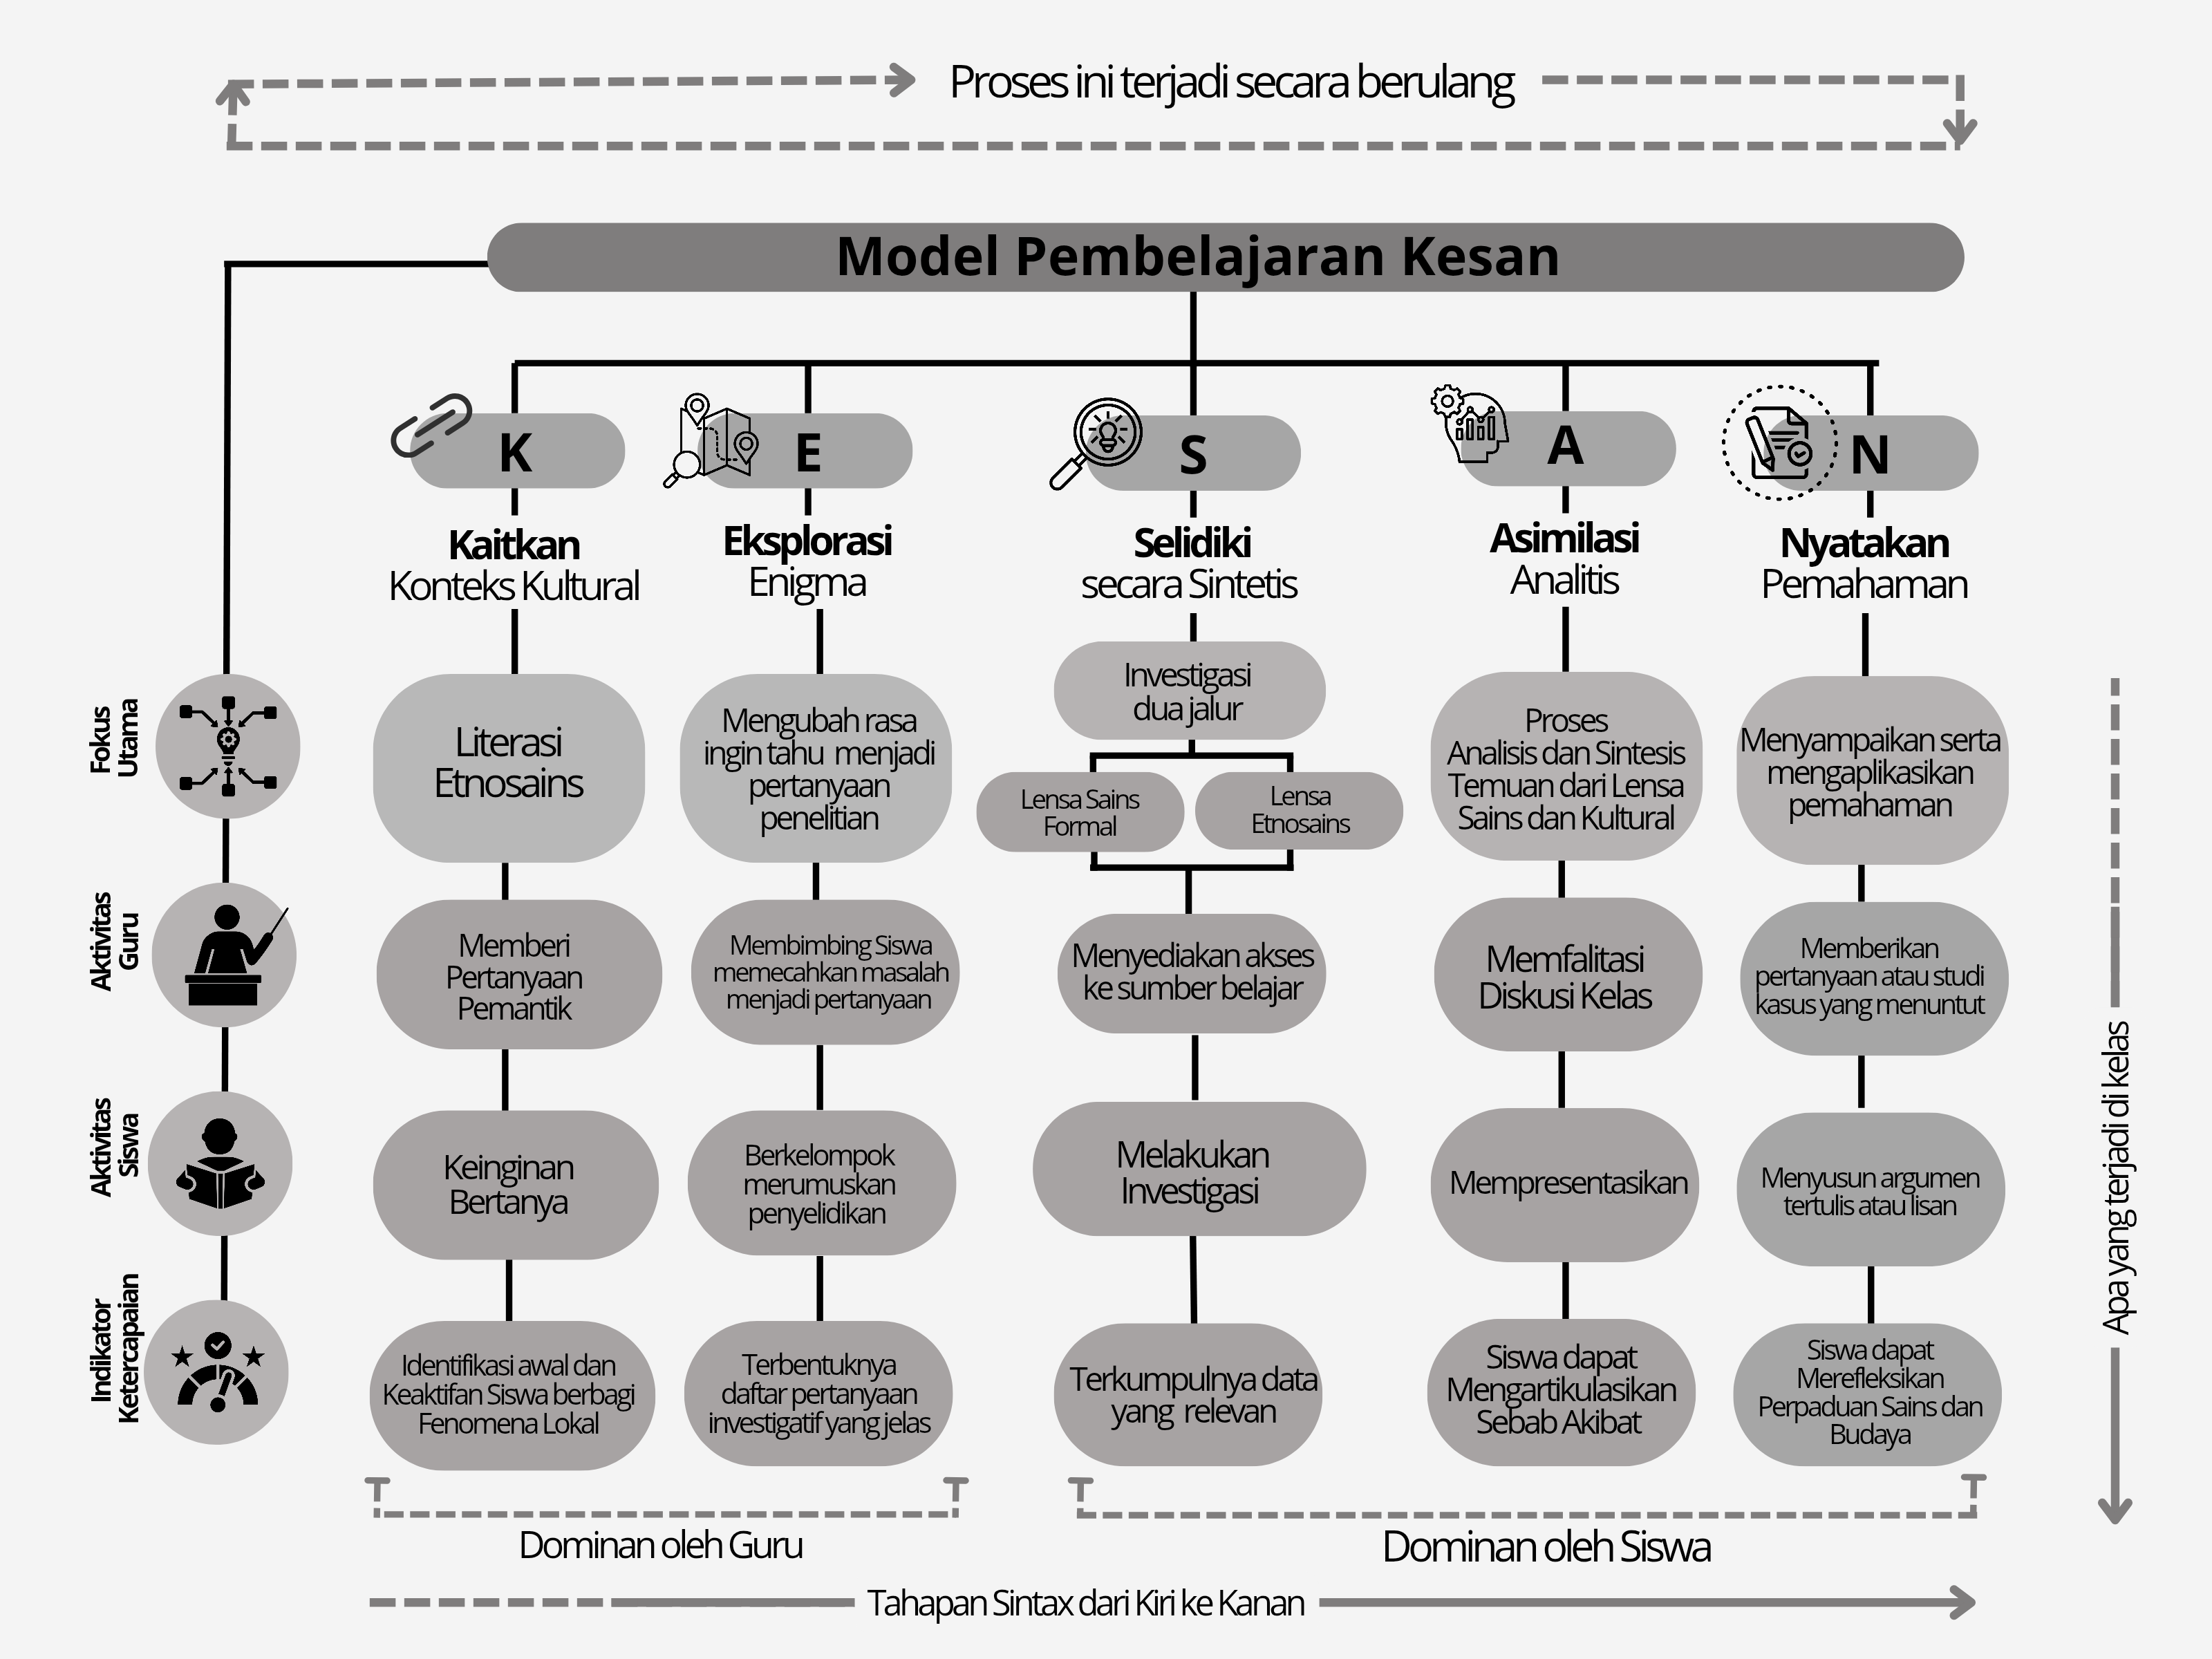
\includegraphics[width=1.1\textwidth]{kesanB.png}
\caption{Panduan Operasional Pelaksanaan Model KESAN untuk Guru}
\label{fig:kesanB}
\end{figure}

\clearpage

\subsection{Pelaksanaan Siklus Pembelajaran Model KESAN}

Untuk menerapkan Model KESAN secara efektif, guru perlu memandang Gambar \ref{fig:kesanA} bukan sebagai diagram statis, melainkan sebagai peta dinamis yang memandu jalannya pembelajaran. Peta ini menunjukkan alur utama sekaligus fleksibilitas yang menjadi kunci keberhasilan model ini.

\begin{figure}[H]
\centering
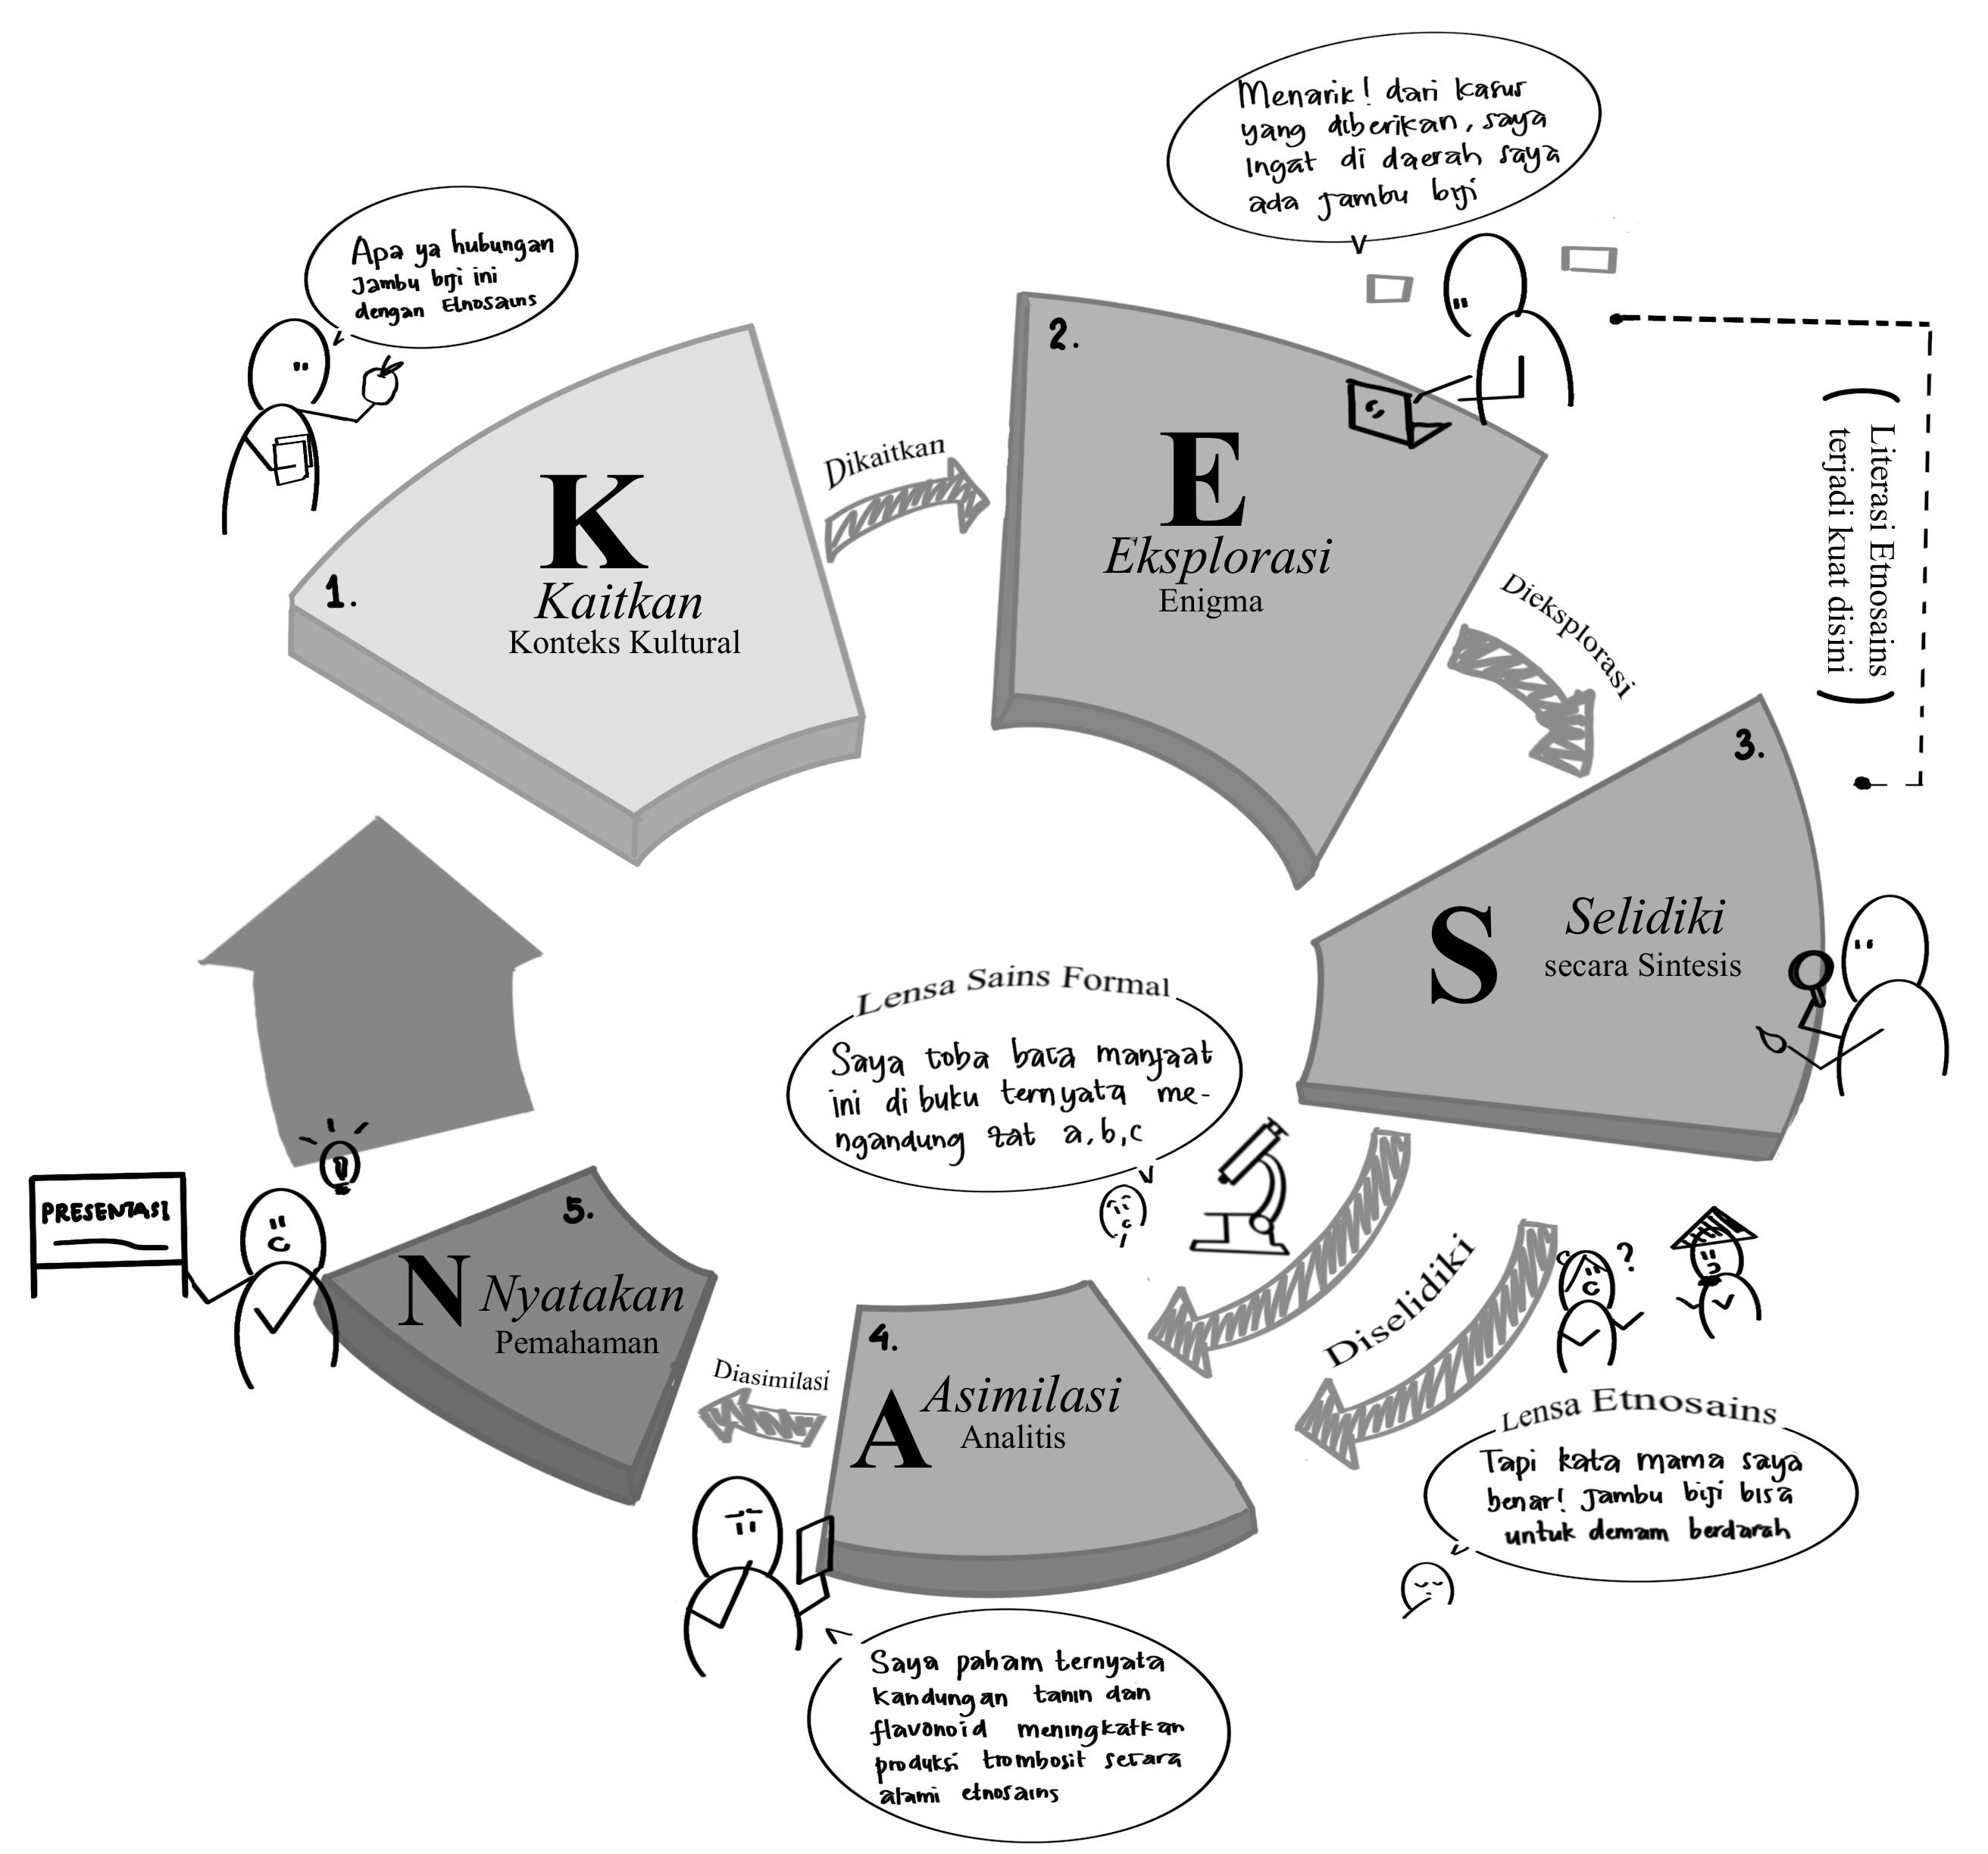
\includegraphics[width=0.85\textwidth]{kesanA.jpg}
\caption{Siklus Pelaksanaan Model KESAN dalam Pembelajaran}
\label{fig:kesanA}
\end{figure}

\textbf{Cara Menggunakan Peta Siklus KESAN:}

Peta ini membantu guru dalam tiga hal utama: menavigasi alur, mengelola fleksibilitas, dan mengukur kesiapan siswa.

\textbf{1. Menavigasi Alur Utama (Panah Maju):}
Setiap tahap adalah sebuah gerbang yang harus dilalui secara berurutan untuk membangun pemahaman yang utuh.
\begin{itemize}
    \item \textbf{K (Kaitkan):} Anggap ini sebagai "gerbang masuk". Tujuan Anda adalah membuka pintu rasa ingin tahu siswa dengan menghubungkan materi ke dunia mereka. \textbf{Tips:} Gunakan objek nyata, cerita lokal, atau video singkat yang relevan. Hindari penjelasan ilmiah di tahap ini.
    \item \textbf{E (Eksplorasi):} Di sini, Anda memandu siswa untuk mengubah rasa ingin tahu menjadi pertanyaan-pertanyaan spesifik. \textbf{Tips:} Gunakan teknik "Question Formulation Technique" (QFT) atau sediakan kerangka pertanyaan untuk membantu siswa.
    \item \textbf{S (Selidiki):} Ini adalah "fase ekspedisi". Siswa mencari jawaban atas pertanyaan mereka dari dua sumber: sains dan budaya. \textbf{Tips:} Siapkan sumber belajar yang beragam dan mudah diakses. Peran Anda adalah sebagai kurator, bukan penceramah.
    \item \textbf{A (Asimilasi):} Fase "negosiasi makna". Di sinilah temuan dari dua jalur dipertemukan. \textbf{Tips:} Gunakan papan tulis atau alat kolaborasi digital untuk memvisualisasikan titik temu dan perbedaan antara kedua perspektif.
    \item \textbf{N (Nyatakan):} Puncak perjalanan, di mana siswa "menceritakan" pemahaman baru mereka. \textbf{Tips:} Berikan tantangan autentik seperti membuat poster, video penjelasan, atau presentasi untuk di kelas.
\end{itemize}
\textbf{2. Mengelola Fleksibilitas (Panah Mundur):}
Panah yang mengarah ke belakang adalah fitur paling kuat dari model ini. Gunakan ini sebagai "tombol reset" strategis.
\begin{itemize}
    \item \textbf{Kapan kembali dari S ke E?} Jika saat investigasi (S), siswa terlihat bingung atau data yang ditemukan tidak relevan. Ini tandanya pertanyaan penelitian (E) mereka kurang fokus. Ajak mereka kembali untuk mempertajam pertanyaan.
    \item \textbf{Kapan kembali dari E ke K?} Jika siswa kesulitan merumuskan pertanyaan (E), kemungkinan koneksi emosional dan kontekstual di tahap K kurang kuat. Kembali ke tahap K untuk menggali lagi relevansi budaya dari topik tersebut.
\end{itemize}

\textbf{3. Indikator Kesiapan Pindah Tahap:}
Gunakan ini sebagai *checklist* sebelum melanjutkan.
\begin{itemize}
    \item \textbf{Siap meninggalkan K:} Siswa secara aktif berbagi cerita dan mulai bertanya "mengapa?" secara spontan.
    \item \textbf{Siap meninggalkan E:} Setiap kelompok telah menghasilkan daftar pertanyaan yang jelas dan dapat diinvestigasi.
    \item \textbf{Siap meninggalkan S:} Kelompok telah mengumpulkan informasi yang cukup dari kedua lensa (sains dan budaya).
    \item \textbf{Siap meninggalkan A:} Siswa mampu merangkai sebuah penjelasan yang menghubungkan konsep sains dengan praktik budaya.
\end{itemize}

\subsection{Panduan Praktis Pelaksanaan per Tahap}

Gunakan panduan ini sebagai rubrik untuk merancang, melaksanakan, dan merefleksikan pembelajaran Anda. Setiap tahap dirancang untuk mencapai tujuan pembelajaran yang spesifik sambil membangun fondasi untuk tahap berikutnya.

\textbf{Tahap K: Kaitkan}
\begin{itemize}
    \item \textbf{Aksi Guru:} Sajikan fenomena budaya (misal: proses pembuatan gula aren). Ajukan pertanyaan pemantik: "Siapa yang pernah melihat ini? Menurut orang tua kalian, kenapa harus diaduk terus-menerus?"
    \item \textbf{Aksi Siswa yang Diharapkan:} Siswa berbagi pengalaman, menceritakan apa yang mereka ketahui dari keluarga, dan menunjukkan antusiasme.
    \item \textbf{Indikator Kunci:} Kelas menjadi hidup dengan cerita-cerita personal. Muncul pertanyaan-pertanyaan awal yang didasari rasa ingin tahu.
    \item \textbf{Tips Anti Gagal:} Jangan terburu-buru menjelaskan konsep "karamelisasi" atau "titik didih". Fokus penuh pada validasi pengalaman siswa.
\end{itemize}

\textbf{Tahap E: Eksplorasi}
\begin{itemize}
    \item \textbf{Aksi Guru:} Fasilitasi diskusi kelompok untuk merumuskan pertanyaan dari fenomena tadi. "Mari kita buat daftar pertanyaan tentang proses pembuatan gula aren tadi."
    \item \textbf{Aksi Siswa yang Diharapkan:} Berdiskusi, berdebat, dan menuliskan pertanyaan seperti: "Apa fungsi api harus stabil? Kenapa warna nira berubah?"
    \item \textbf{Indikator Kunci:} Terbentuknya daftar pertanyaan spesifik di setiap kelompok.
    \item \textbf{Tips untuk Guru:} Sediakan kertas plano atau papan tulis digital agar setiap kelompok dapat memajang pertanyaan mereka. Ini menciptakan rasa kepemilikan.
\end{itemize}

\textbf{Tahap S: Selidiki}
\begin{itemize}
    \item \textbf{Aksi Guru:} Sediakan dua jenis sumber: (1) Artikel/video tentang perubahan kimia pada pemanasan sukrosa. (2) Wawancara dengan pengrajin gula aren atau artikel etnografi.
    \item \textbf{Aksi Siswa yang Diharapkan:} Dalam kelompok, sebagian siswa membaca sumber ilmiah, sebagian lagi mempelajari sumber budaya. Kemudian mereka saling berbagi temuan.
    \item \textbf{Indikator Kunci:} Siswa dapat menjelaskan proses pembuatan gula aren dari dua sudut pandang yang berbeda secara terpisah.
    \item \textbf{Tips Manajemen Kelas:} Gunakan strategi "Jigsaw" di mana setiap siswa menjadi "ahli" untuk satu sumber dan kemudian mengajarkannya kepada teman sekelompok.
\end{itemize}

\textbf{Tahap A: Asimilasi}
\begin{itemize}
    \item \textbf{Aksi Guru:} Lontarkan pertanyaan sintesis: "Sekarang, mari kita hubungkan. Bagaimana konsep 'penguapan air' dari sains menjelaskan mengapa pengrajin menggunakan wajan yang besar dan terbuka?"
    \item \textbf{Aksi Siswa yang Diharapkan:} Terlibat dalam diskusi yang hidup, mencoba menghubungkan istilah ilmiah (laju penguapan) dengan praktik tradisional (bentuk wajan).
    \item \textbf{Indikator Kunci:} Siswa mampu membuat pernyataan seperti: "Oh, jadi wajan besar itu untuk memperluas permukaan agar air cepat menguap, sesuai prinsip sains."
    \item \textbf{Tips Fasilitasi:} Biarkan ada keheningan. Beri siswa waktu untuk berpikir dan memproses sebelum menjawab. Jangan langsung memberikan jawaban.
\end{itemize}

\textbf{Tahap N: Nyatakan}
\begin{itemize}
    \item \textbf{Aksi Guru:} Berikan tugas aplikasi: "Rancanglah sebuah infografis yang menjelaskan sains di balik pembuatan gula aren untuk dipasang di balai desa."
    \item \textbf{Aksi Siswa yang Diharapkan:} Bekerja sama untuk membuat produk yang menunjukkan pemahaman terintegrasi mereka, menggunakan bahasa yang mudah dipahami masyarakat.
    \item \textbf{Indikator Kunci:} Produk akhir siswa secara akurat menggabungkan penjelasan ilmiah dan menghargai kearifan lokal.
    \item \textbf{Tips Penilaian:} Gunakan rubrik penilaian yang mencakup dua aspek: (1) Akurasi konsep sains, dan (2) Kedalaman pemahaman dan penghargaan terhadap konteks budaya.
\end{itemize}

\subsection{Panduan Lanjutan untuk Tahap Kritis}

Dua tahap yang sering menjadi tantangan bagi guru adalah Tahap A (Asimilasi) dan Tahap N (Nyatakan), karena memerlukan keterampilan fasilitasi yang lebih canggih.

\textbf{Tahap A (Asimilasi Analitis)}
\begin{itemize}
\item \textbf{Moderasi Dialog:} Peran guru sangat krusial sebagai moderator yang netral. Gunakan pertanyaan pemicu seperti "Bagaimana temuan dari lensa sains dapat menjelaskan praktik budaya yang kalian temukan?".
\item \textbf{Teknik Sintesis:} Gunakan graphic organizer seperti Venn diagram atau concept mapping untuk membantu siswa melihat koneksi dan perbedaan.
\item \textbf{Indikator Keberhasilan:} Siswa mampu menciptakan narasi baru yang mengintegrasikan kedua perspektif tanpa mengorbankan salah satunya.
\item \textbf{Assessment Criteria:} Evaluasi berdasarkan koherensi argumen, penggunaan evidence dari kedua sumber, dan originalitas sintesis.
\end{itemize}

\textbf{Tahap N (Nyatakan Pemahaman)}
\begin{itemize}
\item \textbf{Desain Challenge:} Berikan authentic assessment berupa studi kasus atau design challenge yang mengharuskan aplikasi pemahaman terintegrasi.
\item \textbf{Scaffolding Refleksi:} Gunakan reflective prompts seperti "Apa yang berubah dalam cara kalian memahami fenomena ini?", "Bagaimana pengetahuan tradisional memperkaya pemahaman sains kalian?".
\item \textbf{Indikator Keberhasilan:} Siswa dapat mengaplikasikan pemahaman untuk konteks baru, menunjukkan transfer knowledge yang bermakna.
\item \textbf{Documentation:} Dokumentasikan produk siswa sebagai evidence pembelajaran dan portfolio untuk assessment formatif.
\end{itemize}

\subsection{Tips Pengelolaan Kelas dan Diferensiasi}

\begin{enumerate}
\item \textbf{Untuk Siswa dengan Prior Knowledge Tinggi:} Berikan peran sebagai peer tutor atau challenger yang mengajukan pertanyaan kritis.
\item \textbf{Untuk Siswa dengan Latar Belakang Budaya Berbeda:} Manfaatkan keberagaman sebagai kekayaan, bukan hambatan. Dorong sharing perspektif budaya yang berbeda.
\item \textbf{Untuk Siswa yang Kurang Aktif:} Gunakan strategi think-pair-share dan berikan tanggung jawab spesifik dalam kelompok.
\item \textbf{Pengelolaan Waktu:} Siapkan plan B untuk setiap tahap jika waktu tidak mencukupi. Tahap S biasanya memerlukan waktu paling banyak.
\end{enumerate}

\chapter{IMPLIKASI DAN PENGEMBANGAN LANJUT}

Setiap inovasi dalam pendidikan tidak berhenti pada titik finalisasinya. Nilai sejatinya justru terletak pada implikasi yang ditimbulkannya serta potensi untuk terus berkembang dan menginspirasi gagasan-gagasan baru. Bab ini akan menarik benang merah dari seluruh pembahasan untuk merumuskan implikasi teoretis dan praktis dari Model KESAN. Lebih dari itu, bab ini juga secara jujur mengakui adanya keterbatasan dan memberikan rekomendasi konstruktif untuk penelitian dan pengembangan lebih lanjut. Tujuannya adalah untuk menempatkan Model KESAN dalam sebuah dialog berkelanjutan dengan komunitas akademik dan para praktisi pendidikan.

\section{Implikasi Teoretis}

Kehadiran Model KESAN membawa serangkaian implikasi yang melampaui sekadar metode pengajaran alternatif. Model ini menawarkan kontribusi bagi wacana teoretis dalam ilmu pendidikan dan secara bersamaan memberikan dampak praktis yang signifikan bagi ekosistem sekolah.

1.  \textbf{Rekonseptualisasi Hubungan antara Pengetahuan Universal dan Lokal:}
    Secara teoretis, kontribusi utama Model KESAN adalah menawarkan sebuah kerangka operasional untuk mendialogkan dua sistem epistemologi—sains Barat modern dan etnosains—dalam posisi yang simetris, bukan hierarkis. Model ini menantang pandangan positivistik yang sering kali menempatkan sains sebagai satu-satunya cara yang valid untuk memahami dunia. Dengan menyediakan sintaks "investigasi dua jalur" yang sistematis, KESAN secara teoretis mengukuhkan bahwa pengetahuan yang tersemat dalam budaya (\textit{culturally embedded knowledge}) bukan sekadar "konsepsi awal" yang perlu dikoreksi, melainkan sebuah korpus pengetahuan yang kaya, yang dapat berdialog, saling memperkaya, dan terkadang mengkritisi narasi sains universal. Ini memberikan sumbangan pada bidang filsafat pendidikan dan sosiologi pengetahuan.

2.  \textbf{Implementasi Konkret Etnosains dalam Pembelajaran:}
Model KESAN memberikan salah satu contoh paling konkret dan terstruktur tentang bagaimana etnosains dapat diintegrasikan dalam pembelajaran sains formal. Ia bergerak dari sekadar "responsif budaya" menuju tindakan "melestarikan dan mengembangkan etnosains" dengan menjadikan etnosains sebagai subjek analisis yang setara dengan sains formal. Model ini membuktikan bahwa tujuan pelestarian identitas budaya dan pencapaian kompetensi akademis bukanlah dua hal yang terpisah, melainkan dapat dicapai secara simultan melalui desain pedagogis yang tepat.

\subsection{Implikasi Praktis}

Tabel \ref{tab:implikasi_praktis} merangkum implikasi praktis Model KESAN bagi berbagai stakeholder pendidikan.

\begin{table}[H]
\centering
\caption{Implikasi Praktis Model KESAN}
\label{tab:implikasi_praktis}
\begin{tabular}{|p{3cm}|p{5cm}|p{6cm}|}
\hline
\textbf{Stakeholder} & \textbf{Dampak Utama} & \textbf{Indikator Keberhasilan} \\
\hline
Peserta Didik & Identitas hibrida yang kuat & Kemampuan navigasi budaya-sains, rasa memiliki, pemberdayaan \\
\hline
Guru & Pengembangan profesional kontekstual & Menjadi peneliti lokal, ko-designer kurikulum \\
\hline
Sekolah & Kurikulum yang berakar & Integrasi dengan komunitas, relevansi kontekstual \\
\hline
Masyarakat & Revitalisasi budaya lokal & Apresiasi terhadap kearifan lokal, dialog intergenerasi \\
\hline
\end{tabular}
\end{table}

1.  \textbf{Bagi Peserta Didik: Menumbuhkan "Identitas Hibrida" yang Kuat:}
    Implementasi KESAN secara langsung berdampak pada pembentukan identitas siswa. Mereka belajar untuk menjadi "penyeberang batas budaya" (\textit{border crossers}) yang fasih. Mereka mampu menavigasi dunia sains modern tanpa harus meninggalkan atau merasa minder dengan akar budayanya. Mereka menjadi individu dengan "identitas hibrida" yang positif: seorang pemikir ilmiah yang juga bangga menjadi bagian dari komunitas budayanya. Dampak afektif ini—rasa memiliki (\textit{sense of belonging}), relevansi (\textit{sense of relevance}), dan pemberdayaan (\textit{sense of agency})—merupakan prasyarat fundamental bagi keterlibatan dan prestasi akademis yang berkelanjutan.

2.  \textbf{Bagi Guru: Mendorong Pengembangan Profesional yang Kontekstual:}
    Model KESAN menuntut guru untuk menjadi seorang peneliti di lingkungannya sendiri. Untuk dapat mengimplementasikan model ini secara efektif, guru didorong untuk belajar lebih banyak tentang budaya lokal, berinteraksi dengan komunitas di luar sekolah, dan secara kreatif mencari hubungan antara kurikulum nasional dengan konteks lokal. Proses ini secara inheren merupakan bentuk pengembangan profesional yang otentik dan berkelanjutan. Guru tidak lagi hanya menjadi konsumen kurikulum, tetapi menjadi \textbf{ko-desainer kurikulum} yang kontekstual.

3.  \textbf{Bagi Sekolah dan Kurikulum: Menuju "Kurikulum yang Berakar":}
    Pada tingkat kelembagaan, adopsi luas Model KESAN dapat membantu sekolah mengembangkan apa yang bisa disebut sebagai "kurikulum yang berakar" (\textit{rooted curriculum}). Artinya, sementara sekolah tetap mengacu pada standar nasional, implementasinya menjadi sangat khas dan unik sesuai dengan konteks ekologis dan budaya di sekitarnya. Sekolah tidak lagi menjadi "menara gading" yang terpisah dari masyarakat, tetapi menjadi pusat pembelajaran yang hidup dan terintegrasi dengan denyut nadi komunitasnya. Hal ini secara langsung menjawab ruh dari kebijakan Kurikulum Merdeka yang menekankan fleksibilitas dan relevansi kontekstual.

\section{Limitasi dan Rekomendasi}

Tidak ada satu pun model pembelajaran yang sempurna atau cocok untuk semua situasi. Sebagai sebuah karya pengembangan yang lahir dari konteks spesifik, Model KESAN memiliki keterbatasan yang perlu diakui secara transparan. Pengakuan ini bukan untuk mengurangi nilainya, melainkan untuk membuka ruang bagi perbaikan dan penelitian di masa depan.

\subsection{Limitasi Model KESAN}

Tabel \ref{tab:limitasi_kesan} mengidentifikasi limitasi utama Model KESAN beserta strategi mitigasinya.

\begin{table}[H]
\centering
\caption{Limitasi Model KESAN dan Strategi Mitigasi}
\label{tab:limitasi_kesan}
\begin{tabular}{|p{4cm}|p{5cm}|p{5cm}|}
\hline
\textbf{Limitasi} & \textbf{Dampak} & \textbf{Strategi Mitigasi} \\
\hline
Intensitas Persiapan Guru & Beban kerja tinggi, resistensi implementasi & Kolaborasi guru, bank sumber belajar, pelatihan bertahap \\
\hline
Cakupan Konsep Sains & Tidak semua topik cocok & Seleksi topik strategis, adaptasi kreatif, kombinasi metode \\
\hline
Ketersediaan Sumber Budaya & Dokumentasi budaya terbatas & Kemitraan dengan komunitas, digitalisasi kearifan lokal \\
\hline
Penilaian Standar & Konflik dengan tes nasional & Asesmen alternatif, portofolio, rubrik holistik \\
\hline
\end{tabular}
\end{table}

1.  \textbf{Intensitas Persiapan Guru:} Implementasi Model KESAN yang berkualitas menuntut waktu dan upaya persiapan yang signifikan dari guru, terutama dalam fase perencanaan untuk memilih konteks dan mengurasi sumber belajar. Dalam sistem di mana guru dibebani dengan tugas administrasi yang berat, hal ini dapat menjadi hambatan praktis yang substansial.

2.  \textbf{Cakupan Konsep Sains:} Tidak semua konsep sains dapat dengan mudah dihubungkan dengan fenomena budaya yang kasatmata. Konsep-konsep yang sangat abstrak atau berada pada skala mikroskopis (seperti fisika kuantum atau genetika molekuler tingkat lanjut) mungkin lebih menantang untuk diimplementasikan melalui alur KESAN yang otentik. Model ini paling efektif untuk topik-topik yang memiliki manifestasi makroskopis dalam kehidupan sehari-hari.

3.  \textbf{Potensi Romantisasi Budaya:} Jika tidak difasilitasi dengan kritis, ada risiko bahwa model ini dapat mengarah pada romantisasi budaya lokal, mengabaikan aspek-aspek yang mungkin problematis atau tidak lagi relevan. Peran guru sebagai fasilitator yang kritis (seperti yang disarankan dalam revisi model) menjadi sangat krusial untuk mencegah hal ini, namun menuntut tingkat kematangan pedagogis yang tinggi.

4.  \textbf{Ketergantungan pada Sumber Daya Kontekstual:} Efektivitas model sangat bergantung pada kekayaan konteks budaya dan ketersediaan sumber daya (termasuk narasumber) di lingkungan sekolah. Di lingkungan urban yang sangat heterogen dan mungkin telah kehilangan banyak jejak kearifan lokal spesifik, guru mungkin memerlukan kreativitas ekstra untuk menemukan konteks yang otentik.

\subsection{Rekomendasi untuk Pengembangan dan Penelitian Lanjut}

Berdasarkan implikasi dan limitasi di atas, Tabel \ref{tab:rekomendasi_lanjut} menyajikan arah pengembangan dan penelitian di masa depan.

\begin{table}[H]
\centering
\caption{Rekomendasi Pengembangan dan Penelitian Lanjut Model KESAN}
\label{tab:rekomendasi_lanjut}
\begin{tabular}{|p{4cm}|p{5cm}|p{5cm}|}
\hline
\textbf{Area Pengembangan} & \textbf{Fokus Utama} & \textbf{Output yang Diharapkan} \\
\hline
Bank Konteks Digital & Platform kolaboratif sumber budaya-sains & Repositori konteks terintegrasi kurikulum \\
\hline
Adaptasi Lintas Disiplin & Implementasi di IPS, Matematika, Bahasa & Model adaptasi untuk berbagai mata pelajaran \\
\hline
Studi Longitudinal & Dampak jangka panjang terhadap identitas & Data pembentukan identitas keilmuan-budaya \\
\hline
Integrasi Teknologi Imersif & AR/VR untuk konteks budaya & Pengalaman virtual kearifan lokal \\
\hline
Pelatihan Guru Berkelanjutan & Kompetensi fasilitasi dialog kritis & Program sertifikasi guru KESAN \\
\hline
\end{tabular}
\end{table}

Beberapa arah pengembangan dan penelitian di masa depan sangat direkomendasikan:

1.  \textbf{Pengembangan Bank Konteks Digital:} Untuk mengatasi masalah intensitas persiapan guru, perlu dikembangkan sebuah platform atau bank sumber belajar digital secara kolaboratif. Platform ini dapat berisi koleksi konteks budaya, kearifan lokal, dan fenomena dari berbagai daerah di Indonesia, yang sudah dipetakan dengan konsep-konsep sains yang relevan dalam kurikulum. Guru dari seluruh Indonesia dapat berkontribusi dan menggunakan sumber daya ini.

2.  \textbf{Penelitian tentang Adaptasi Lintas Disiplin:} Diperlukan penelitian lebih lanjut yang secara sistematis menguji efektivitas adaptasi Model KESAN di luar bidang sains, seperti dalam studi sosial, matematika (etnomatematika), dan bahasa. Studi komparatif dapat mengidentifikasi bagaimana sintaks dan prinsip model perlu disesuaikan untuk setiap bidang ilmu.

3.  \textbf{Studi Longitudinal Mengenai Dampak Identitas:} Penelitian yang ada saat ini umumnya berjangka pendek. Studi longitudinal selama beberapa tahun akan sangat berharga untuk melacak dampak jangka panjang dari pembelajaran berbasis KESAN terhadap pilihan karier, partisipasi komunitas, dan pembentukan identitas keilmuan-kebudayaan siswa hingga mereka dewasa.

4.  \textbf{Integrasi dengan Teknologi Imersif:} Menjelajahi bagaimana teknologi baru seperti \textit{Augmented Reality} (AR) dan \textit{Virtual Reality} (VR) dapat memperkaya implementasi KESAN. Misalnya, siswa di kota dapat "mengunjungi" secara virtual proses pembuatan perahu tradisional di pesisir, memungkinkan akses ke konteks yang jauh secara geografis.

Pada akhirnya, Model Pembelajaran KESAN bukanlah sebuah kata akhir, melainkan sebuah kalimat pembuka. Ia adalah sebuah undangan terbuka bagi para pendidik, peneliti, dan pembuat kebijakan untuk bersama-sama terus berinovasi, memastikan bahwa setiap anak di negeri ini dapat merasakan pengalaman belajar yang tidak hanya mencerdaskan pikiran, tetapi juga menghangatkan jiwa dan menguatkan akar identitasnya.

\begin{thebibliography}{99}
\bibitem{ausubel} Ausubel, D. P. (1968). \textit{Educational psychology: A cognitive view}. Holt, Rinehart and Winston.

\bibitem{vygotsky} Vygotsky, L. S. (1978). \textit{Mind in society: The development of higher psychological processes}. Harvard University Press.



\bibitem{aikenhead} Aikenhead, G. S., & Jegede, O. J. (1999). Cross-cultural science education: A cognitive explanation of a cultural phenomenon. \textit{Journal of Research in Science Teaching, 36}(3), 269-287.

\bibitem{plomp} Plomp, T. (2013). Educational design research: An introduction. In T. Plomp & N. Nieveen (Eds.), \textit{Educational design research – Part A: An introduction} (pp. 10-51). SLO.

\bibitem{rose} Rose, D., & Martin, J. R. (2012). \textit{Learning to write, reading to learn: Genre, knowledge and pedagogy in the Sydney School}. Equinox.



\bibitem{zeidler} Zeidler, D. L., Sadler, T. D., Simmons, M. L., & Howes, E. V. (2005). Beyond STS: A research-based framework for socioscientific issues education. \textit{Science Education, 89}(3), 357-377.

\bibitem{nieveen} Nieveen, N. (1999). Prototyping to reach product quality. In J. van den Akker, R. M. Branch, K. Gustafson, N. Nieveen, & T. Plomp (Eds.), \textit{Design approaches and tools in education and training} (pp. 125-136). Springer.

\bibitem{ladson} Ladson-Billings, G. (1995). Toward a theory of culturally relevant pedagogy. \textit{American Educational Research Journal, 32}(3), 465-491.
\end{thebibliography}

\appendix
\chapter{INSTRUMEN EVALUASI}
\chapter{CONTOH IMPLEMENTASI}
\end{document}